\documentclass[device=normal, lang=en]{elegantbook}
\usepackage{amsmath}
\usepackage{amssymb}
\usepackage{float}
\usepackage{extarrows}
\usepackage{physics}
\usepackage{mathtools}
\usepackage{tikz}
\usepackage[inkscapelatex=false]{svg}

\newcommand{\e}{\mathrm{e}}


\definecolor{pgcolor}{RGB}{251, 250, 248}
\pagecolor{pgcolor}
\numberwithin{equation}{section}

% \theoremstyle{definition} %
% \newtheorem{property}{Property}[section] %

\title{Probability Notes}
\author{FHYQ-Dong}
\date{\today}
\version{13.0}
\cover{images/Note-cover.png}
\definecolor{customcoverlinecolor}{RGB}{82, 59, 148}
\colorlet{coverlinecolor}{customcoverlinecolor}


\begin{document}

\maketitle
\frontmatter

\tableofcontents
\mainmatter


\chapter{Probability Space}
\begin{definition}[Probability Space]
    Probability space is a tuple $\left(\varOmega,~\mathcal{F},~\mathbf{P}\right)$ where
    \begin{itemize}
        \item Sample space $\varOmega$ is a set of all possible outcomes.
        \item $ \sigma $-algebra $\mathcal{F}$ is a collection of subsets of $\varOmega$.
        \item Probability measure $\mathbf{P}$ is a function that assigns a probability to each event in $\mathcal{F}$.
    \end{itemize}
\end{definition}

\begin{definition}[Sample Space]
    Sample space $\varOmega$ is a set of all possible outcomes, which should satisfy the following properties:
    \begin{itemize}
        \item Mutually Exclusive: The elements in $\varOmega$ should be unique.
        \item Collectively Exhaustive: The elements in $\varOmega$ should cover all possible outcomes.
    \end{itemize}
\end{definition}

Once the experiment is conducted, there is \textbf{exactly one} element in the sample space $\varOmega$ occurs.

\begin{example}[Example of Sample Space]
    Here are some examples of sample space:
    \begin{itemize}
        \item Discrete: $\varOmega = \{1, 2, 3, 4, 5, 6\}$ - Rolling a fair die.
        \item Continuous: $\varOmega = [0, 1]$ - Randomly selecting a real number between 0 and 1.
    \end{itemize}
\end{example}

Before we define the $\sigma$-algebra, we need to introduce the concept of \textbf{countable}. We say a set $X$ is countable if there is a bijection between $X$ and $\mathbb{N}$. Some countable sets are: $\mathbb{N}$, $\mathbb{Z}$, $\mathbb{Q}$, $\mathbb{N}^2$, $\mathbb{Z}^2$, $\mathbb{Q}^2$, $\cup_{n=1}X_{n}$. Some uncountable sets are: $\mathbb{R}$, $\mathbb{C}$, $\mathbb{R}^2$, $\mathbb{C}^2$.

\begin{definition}[$\sigma$-algebra]
    We say a set $\mathcal{F}$  collection of subsets of $\varOmega$ is a $\sigma$-algebra if it satisfies the following properties:
\end{definition}

\begin{remark}
    Not all the things in real worlf can be measured by probability, especially when things are continuous (uncountable).
\end{remark}

\chapter{Conditional Probability}
\section{Conditional Probability}
\begin{definition}[Conditional Probability]
    Conditional probability is the probability of an event $A$ given that another event $B$ has already occurred. It is denoted by $P(A|B)$ and is defined as:
    \begin{equation}
        \mathbf{P}(A|B) = \frac{\mathbf{P}(A \cap B)}{\mathbf{P}(B)}
    \end{equation}
    Note that when $\mathbf{P}(B) = 0$, the conditional probability is undefined.
\end{definition}

We can easily check the conditional probability satisfies the properties of probability measure, which means it is a legitimate probability on a new universe.
\begin{itemize}
    \item Non-negativity: $\mathbf{P}(A|B) \geq 0$.
    \item Normalization: $\mathbf{P}(\varOmega|B) = 1$.
    \item Additivity: when $A$ and $B$ are disjoint, $\mathbf{P}(A \cup B|C) = \frac{\mathbf{P}((A \cup B) \cap C)}{\mathbf{P}(C)} = \frac{\mathbf{P}(A \cap C) + \mathbf{P}(B \cap C)}{\mathbf{P}(C)} = \mathbf{P}(A|C) + \mathbf{P}(B|C)$. (The second equality is due to $A \cap C$ and $B \cap C$ are disjoint).
\end{itemize}

\begin{example}[Discrete and Continuous]
    For discrete case, the conditional probability can be calulated by:
    \begin{equation}
        \mathbf{P}(A|B) = \frac{\#~of~elements~in~A}{\#~of~elements~in~B}
    \end{equation}
    For continuous case, the conditional probability can be calculated by:
    \begin{equation}
        \mathbf{P}(A|B) = \frac{area~of~A}{area~of~B}
    \end{equation}
\end{example}

When solving a problem, the following equations may help:
\begin{align}
    \mathbf{P}(A \cap D) &= \mathbf{P}(A) \cdot \mathbf{P}(D|A) \\
    &= \mathbf{P}(D) \cdot \mathbf{P}(A|D) \\
    \mathbf{P}(A \cap B \cap C) &= \mathbf{P}(A) \cdot \mathbf{P}(B|A) \cdot \mathbf{P}(C|A \cap B)
\end{align}
For the second equation: 1.event $A$ occurs; 2.event $B$ occurs given $A$; 3.event $C$ occurs given $A$ and $B$. Or
\begin{align*}
    \mathbf{P}(A \cap B \cap C) &= \mathbf{P}(A \cap B) \cdot \mathbf{P}(C | A \cap B) \\ 
    &= \mathbf{P}(A) \cdot \mathbf{P}(B | A) \cdot \mathbf{P}(C | A \cap B)
\end{align*}
\begin{remark}
    These equations are not fixed, depending on $\mathbf{P}(A)$, $\mathbf{P(A \cap B)}$ and $\mathbf{P}(A | B)$ which are easier to calculate.
\end{remark}

\section{Total Probability Theorem}
We can calculate the total probability with \textit{Devide and Conquer} strategy:
\begin{enumerate}
    \item Devide event $B$ by $A_1, A_2, \cdots A_n$, note that $\bigcup_{i=1}^n A_i = \varOmega$ and $A_i \cap A_j = \emptyset$.
    \item Calculate $\mathbf{P}(B | A_i)$ which are easier to calculate.
    \item Sum all the probabilities.
\end{enumerate}
\begin{figure}[H]
    \centering
    \includegraphics[width=0.3\textwidth]{images/Note-2.1.png}
    \caption{Total Probability Theorem}
    \label{fig:total-probability}
\end{figure}

\begin{theorem}[Total Probability Theorem]
    Let $A_1, A_2, \cdots, A_n$ be a partition of the sample space $\varOmega$. Then for any event $B$,
    \begin{equation}
        \mathbf{P}(B) = \sum_{i=1}^{n} \mathbf{P}(A_i) \cdot \mathbf{P}(B | A_i)
    \end{equation}
\end{theorem}
\begin{example}[Die Rolling]
    You roll a fair four-sided die. If the result is 1 or 2, you roll once more but otherwise, you stop. What is the probability that the sum total of rolls is at least 4?
    \begin{solution}
        \begin{enumerate}
            \item Let $A_i = \{the~first~roll~is~i\}, B = \{the~sum~total~of~rolls~is~at~least~4\}$.
            \item $\mathbf{P}(A_1) = \mathbf{P}(A_2) = \mathbf{P}(A_3) = \mathbf{P}(A_4) = \frac{1}{4}$.
            \item $\mathbf{P}(B | A_1) = \frac{1}{2}, \mathbf{P}(B | A_2) = \frac{3}{4}, \mathbf{P}(B | A_3) = 0, \mathbf{P}(B | A_4) = 1$.
            \item $\mathbf{P}(B) = \frac{9}{16}$.
        \end{enumerate}
    \end{solution}
\end{example}


\section{Bayes' Theorem}
If we know:
\begin{itemize}
    \item ``Prior'' probabilities $\mathbf{P}(A_i)$.
    \item ``Likelihood'' probabilities $\mathbf{P}(B | A_i)$.
\end{itemize}
We wish we can calculate the ``Posterior'' probabilities $\mathbf{P}(A_i | B)$. 

\begin{theorem}[Bayes' Theorem]
    Let $A_1, A_2, \cdots, A_n$ be a partition of the sample space $\varOmega$. Then for any event $B$
    \begin{equation}
    \begin{aligned}
        \mathbf{P}(A_i | B) &= \frac{\mathbf{P}(A_i \cap B)}{\mathbf{P}(B)} \\
        &= \frac{\mathbf{P}(A_i) \cdot \mathbf{P}(B | A_i)}{\sum_{j=1}^{n} \mathbf{P}(A_j) \cdot \mathbf{P}(B | A_j)} \\
        &= \frac{\mathbf{P}(A_i) \cdot \mathbf{P}(B | A_i)}{\sum_{j=1}^{n} \mathbf{P}(A_j) \cdot \mathbf{P}(B | A_j)}
    \end{aligned}
    \end{equation}
\end{theorem}

A: cause, B: result. Bayes' Theorem is used to calculate the cause given the result. \textit{(inference based on probability)}

\chapter{Independence}
\section{Independence}
\begin{definition}[Independence]
    Event $A$ and $B$ are independent if:
    \begin{equation}
        \mathbf{P}(A \cap B) = \mathbf{P}(A) \cdot \mathbf{P}(B)
    \end{equation}
    or equivalently, when $\mathbf{P}(B) \neq 0$:
    \begin{equation}
        \mathbf{P}(A|B) = \mathbf{P}(A)
    \end{equation}
\end{definition}
Occurrence of $B$ does not provides no information about the occurrence of $A$.
\begin{remark}
    Disjoint events are not independent.
    \begin{equation}
    \begin{aligned}
        \mathbf{P}(A \cap B) &= 0 \\
        \mathbf{P}(A \cap B) &= \mathbf{P}(A) \cdot \mathbf{P}(B)
    \end{aligned}
    \end{equation}
    Only if $\mathbf{P}(A) = 0$ or $\mathbf{P}(B) = 0$, the two equations can be both satisfied. E.g. when a student is in one class, it is unlikely that he is in another class.
\end{remark}

\section{Conditional Independence}
\begin{definition}[Conditional Independence]
    Event $A$ and $B$ are conditionally independent given $C$ if:
    \begin{equation}
        \mathbf{P}(A \cap B | C) = \mathbf{P}(A | C) \cdot \mathbf{P}(B | C)
    \end{equation}
\end{definition}
\begin{remark}
    Conditional independence does not imply independence. Information of the mainland of China does not imply the information of Tsinghua University.
\begin{figure}[H]
    \centering
    \includegraphics[width=0.3\textwidth]{images/Note-3.1.png}
    \caption{Conditional Independence}
    \label{fig:conditional-independence}
\end{figure}
As shown in Figure \ref{fig:conditional-independence}, assume $A$ and $B$ are independent. Obviously, $A$ and $B$ are not independent given $C$ (they are disjoint in $C$).
\end{remark}

\section{Independence of Multiple Events}
\begin{definition}[Independence of multiple events]
    Events $A_1, A_2, \cdots, A_n$ are independent if
    \begin{equation}
        \mathbf{P}(A_{i_1} \cap A_{i_2} \cap \cdots \cap A_{i_k}) = \mathbf{P}(A_{i_1}) \cdot \mathbf{P}(A_{i_2}) \cdots \mathbf{P}(A_{i_k})
    \end{equation}
    for any subset $\{i_1, i_2, \cdots, i_k\} \subseteq \{A_1, A_2, \cdots, A_n\}$.
\end{definition}
\begin{remark}
    Pair independence does not imply independence of multiple events. We should check if $\mathbf{P}(\bigcap_{i=1}^{n} A_i) = \prod_{i=1}^{n} \mathbf{P}(A_i)$.
\end{remark}

\chapter{Discrete Random Variables}
\section{Random Variables}
Random variables (RV) is not a variable, but a diterministic function that maps the sample space to the real number, whose range is either finite or countably infinite. Notation: $X(\omega) = x$.
\begin{definition}[Random Variable]
    Given a probability space $(\varOmega, \mathcal{F}, \mathbf{P})$, a random variable $X$ is a function $X: \varOmega \rightarrow \mathbb{R}$ such that for any $x \in \mathbb{R}$, the set $\{\omega \in \varOmega: X(\omega) \leq x\} \in \mathcal{F}$.
\end{definition}
The intuition of introducing RV is to map the sample space to $\mathbb{R}$ so that we can apply some mathmatical tools to analyze the probability distribution of the sample space. But the probability meature on $\mathbb{R}$ is defined on Borel field $\mathcal{B}(\mathbb{R})$, \textbf{so if we want to calculate the probability of RV}, we should consider the a set $A \in \mathcal{B}(\mathbb{R})$. To maintain the consistency between RV and events, the pre-image of $A$ under $X$ should be in $\mathcal{F}$, i.e. for any $x \in \mathbb{R}$, the set $\{\omega \in \varOmega: X(\omega) \leq x\} \in \mathcal{F}$.
\begin{remark}
    The requirement $\forall x \in \mathbb{R},~ \{\omega \in \varOmega: X(\omega) \leq x\} \in \mathcal{F}$ is naturally met when the events in $\varOmega$ are discrete, because we can choose $\mathcal{F} = 2^{\varOmega}$.
\end{remark}
\begin{example}[Examples of RV] ~ \\ 
    A sequence of 5 tosses of a coin:
    \begin{itemize}
        \item The number of heads in the sequence [Discrete RV]
        \item The 5-long sequence is not a RV.
    \end{itemize}
    Two rolls of a die:
    \begin{itemize}
        \item The sum of two rolls [Discrete RV]
        \item The second roll to the power of the first roll [Discrete RV]
    \end{itemize}
    DeepSeek's inference:
    \begin{itemize}
        \item The latency in generating a response [Continuous RV]
        \item The number of requests in a second [Discrete RV]
    \end{itemize}
\end{example}

\section{Probability Mass Function}
\begin{definition}[Probability Mass Function]
    Probability mass function (PMF) is the ``probability law'' or ``probability distribution'' of a \textbf{discrete RV} $X$.
    \begin{align}
        p_{X}(x) &= \mathbf{P}(X = x) = \\ 
                 &= \mathbf{P}(\{\omega \in \varOmega: X(\omega) = x\})
    \end{align}
\end{definition}
Several properties of PMF can be derived from the axioms of probability, e.g. $p_{X}(x) \geq 0$, $\sum_{x} p_{X}(x) = 1$.
\begin{example}[Binomial PMF]
    \begin{align}
        p_{X}(k) &= \binom{n}{k} p^{k} (1-p)^{n-k}
    \end{align}
    One example: the number of heads in $n$ independent tosses of a coin.
\end{example}
\begin{example}[Geometric PMF]
    \begin{align}
        p_{X}(k) &= (1-p)^{k-1} p
    \end{align}
    One example: the number of tosses until the first head appears.
\end{example}
\begin{example}[Poisson PMF]
    \begin{align}
        p_{X}(k) = \mathrm{e}^{-\lambda} \frac{\lambda^{k}}{k!}
    \end{align}
    It's a good approximation of the binomial distribution when $n$ is large and $p$ is small.
    \begin{proof}
        Let $p = \frac{\lambda}{n}$, then
        \begin{align}
            \binom{n}{k} p^{k} (1-p)^{n-k} &= \frac{n!}{k!(n-k)!} p^{k} (1-p)^{n-k} \\
            &= \frac{n(n-1)\cdots(n-k+1)}{k!} p^{k} (1-p)^{n-k} \\
            &\approx \frac{n^{k}}{k!} p^{k} (1-p)^{n-k} \\
            &= \frac{n^{k}}{k!} \left(\frac{\lambda}{n}\right)^{k} \left(1-\frac{\lambda}{n}\right)^{n} \\
            &\approx \frac{n^{k}}{k!} \left(\frac{\lambda}{n}\right)^{k} \mathrm{e}^{-\lambda} \\
            &= \mathrm{e}^{-\lambda} \frac{\lambda^{k}}{k!}
        \end{align}
    \end{proof}
\end{example}
Note that all these PMFs are normalized.

\section{Functions of Random Variables}
\begin{definition}[Function of Random Variables]
    Given a RV $X$, a function $Y = g(X)$ is also a RV. If $X$ is discrete, then $Y$ is also discrete, with PMF $p_{Y}$ given by
    \begin{align}
        p_{Y}(y) = \sum_{x: g(x) = y} p_{X}(x)
    \end{align}
\end{definition}
\begin{remark}
    The function $g$ is defined on $\mathbb{R}$, i.e. $g: \mathbb{R} \rightarrow \mathbb{R}$. The meaning of $Y = g(X)$ in fact is $Y(\omega) = g(X(\omega))$.
\end{remark}

\section{Expectation and Variance}
\begin{definition}[Expectation of Random Variables]
    The expected value (also called the expectation or the mean) of a random variable $X$, with PMF $p_{X}$, is defined as
    \begin{align}
        \mathbf{E}[X] = \sum_{x} x p_{X}(x)
    \end{align}
\end{definition}
While the PMF gives us the full information about the distribution of $X$, sometimes we still need an overall measure of $X$.
\begin{property}[Properties of Expectation] ~ 
    \begin{itemize}
        \item Let $X$ be a RV and $Y = g(X)$. Sometimes $\mathbf{E}[Y] = \sum_{y} y p_{Y}(y)$ is hard to calculate. Instead, we can use $\mathbf{E}[Y] = \sum_{x} g(x) p_{X}(x)$ which is easier.
        \begin{proof}
            \begin{align}
                \mathbf{E}[Y] &= \sum_{y} y p_{Y}(y) \\
                              &= \sum_{y} y \sum_{x: g(x) = y} p_{X}(x) \\
                              &= \sum_{x} g(x) p_{X}(x)
            \end{align}
        \end{proof}
        \item In general, $\mathbf{E}[g(X)] \neq g(\mathbf{E}[X])$.
        \item If $\alpha_1, \alpha_2, \beta$ are constants, $X, Y$ are RVs, then
        \begin{align}
            \mathbf{E}[\alpha_1 X + \alpha_2 Y + \beta] = \alpha_1 \mathbf{E}[X] + \alpha_2 \mathbf{E}[Y] + \beta
        \end{align}
    \end{itemize}
\end{property}
\begin{definition}[Variance of Random Variables]
    The variance of a RV $X$ is defined as
    \begin{align}
        \mathrm{var}(X) = \mathbf{E}[(X - \mathbf{E}[X])^{2}]
    \end{align}
\end{definition}
Remember $\mathbf{E}[g(x)] = \sum_{x} g(x) p_{X}(x)$, then $\mathrm{var}(X) = \sum_{x} (x - \mathbf{E}[X])^{2} p_{X}(x)$.
We can also define the standard deviation as $\sigma(X) = \sqrt{\mathrm{var}(X)}$.
\begin{property}[Properties of Variance] ~ 
    \begin{itemize}
        \item Define second moment as $\mathbf{E}[X^2] = \sum_x x^2 p_{X}(x)$, then $\mathrm{var}(X)$ can be written in terms of moments expression $\mathrm{var}(X) = \mathbf{E}[X^{2}] - \mathbf{E}[X]^{2}$.
        \item $\mathrm{var}(X) \geq 0$.
        \item $\mathrm{var}(\alpha X + \beta) = \alpha^{2} \mathrm{var}(X)$.
    \end{itemize}
\end{property}
\begin{example}[Expectation and Variance of Binomial Distribution]
    \begin{align}
    &\begin{aligned}
        \mathbf{E}[X] &= \sum_{k=0}^{n} k \binom{n}{k} p^{k} (1-p)^{n-k} \\
                      &= \sum_{k=1}^{n} np \binom{n-1}{k-1} p^{k-1} (1-p)^{n-k} \\
                      &= np \sum_{k=1}^{n} \binom{n-1}{k-1} p^{k-1} (1-p)^{n-k} \\
                      &= np \sum_{k=0}^{n-1} \binom{n-1}{k} p^{k} (1-p)^{n-1-k} \\
                      &= np \cdot \mathrm{PMF} = np
    \end{aligned} \\
    &\begin{aligned}
        \mathbf{E}[X^{2}] =& \sum_{k=0}^{n} k^{2} \binom{n}{k} p^{k} (1-p)^{n-k} \\
                         =& np \sum_{k=1}^{n} k \binom{n-1}{k-1} p^{k-1} (1-p)^{n-k} \\
                         =& np \sum_{k=1}^{n} (k-1+1) \binom{n-1}{k-1} p^{k-1} (1-p)^{n-k} \\ 
                         =& n(n-1)p^2 \sum_{k=2}^{n} \binom{n-2}{k-2} p^{k-2} (1-p)^{n-k} \\ 
                         &+ np \sum_{k=1}^{n} (k-1+1) \binom{n-1}{k-1} p^{k-1} (1-p)^{n-k} \\ 
                         =& n(n-1)p^2 + np
    \end{aligned} \\
    &\begin{aligned}
        \mathrm{var}(X) &= \mathbf{E}[X^{2}] - \mathbf{E}[X]^{2} \\
                        &= n(n-1)p^2 + np - n^2p^2 \\
                        &= np(1-p)
    \end{aligned}
    \end{align}
    Let $n = 1$, then the binomial distribution is the Bernoulli distribution.
\end{example}
\begin{example}[Expectation and Variance of Poisson Distribution]
    \begin{align}
    &\begin{aligned}
        \mathbf{E}[X] &= \sum_{k=0}^{\infty} k \mathrm{e}^{-\lambda} \frac{\lambda^{k}}{k!} \\
                      &= \lambda \mathrm{e}^{-\lambda} \sum_{k=1}^{\infty} \frac{\lambda^{k-1}}{(k-1)!} \\
                      &= \lambda \mathrm{e}^{-\lambda} \mathrm{e}^{\lambda} \\
                      &= \lambda
    \end{aligned} \\
    &\begin{aligned}
        \mathbf{E}[X^{2}] &= \sum_{k=0}^{\infty} k^{2} \mathrm{e}^{-\lambda} \frac{\lambda^{k}}{k!} \\
                         &= \lambda \mathrm{e}^{-\lambda} \sum_{k=1}^{\infty} k \frac{\lambda^{k-1}}{(k-1)!} \\
                         &= \lambda \mathrm{e}^{-\lambda} \sum_{k=1}^{\infty} (k-1+1) \frac{\lambda^{k-1}}{(k-1)!} \\
                         &= \lambda \mathrm{e}^{-\lambda} \left(\lambda \sum_{k=1}^{\infty} \frac{\lambda^{k-1}}{(k-1)!} + \sum_{k=1}^{\infty} \frac{\lambda^{k-1}}{(k-1)!}\right) \\
                         &= \lambda \mathrm{e}^{-\lambda} (\lambda \mathrm{e}^{\lambda} + \mathrm{e}^{\lambda}) \\
                         &= \lambda^{2} + \lambda
    \end{aligned} \\
    &\begin{aligned}
        \mathrm{var}(X) &= \mathbf{E}[X^{2}] - \mathbf{E}[X]^{2} \\
                        &= \lambda^{2} + \lambda - \lambda^{2} \\
                        &= \lambda
    \end{aligned}
    \end{align}
\end{example}

\chapter{Multiple Random Variables}
\section{Conditioning}
\begin{definition}[Conditional PMF]
    The conditional PMF of $X$ given $A$ is defined as
    \begin{align}
        p_{X|A}(x) = \mathbf{P}(X = x | A) = \frac{\mathbf{P}(\{X = x\} \cap A)}{\mathbf{P}(A)}
    \end{align}
    Specifically, if given $Y = y$, then
    \begin{align}
        p_{X|Y = y}(x) = \mathbf{P}(X = x | Y = y) = \frac{\mathbf{P}(\{X = x\} \cap \{Y = y\})}{\mathbf{P}(Y = y)}
    \end{align}
\end{definition}
Since $\mathbf{P}(A) = \sum_{x} \mathbf{P}(\{X = x\} \cap A)$, we have $\sum_{x} p_{X|A}(x) = 1$.
The conditional PMF limits the sample space to $A$.
\begin{definition}[Conditional Expectation]
    The conditional expectation of $X$ given $A$ is defined as
    \begin{align}
        \mathbf{E}[X|A] = \sum_{x} x p_{X|A}(x)
    \end{align}
    Specifically, if given $Y = y$, then
    \begin{align}
        \mathbf{E}[X|Y = y] = \sum_{x} x p_{X|Y}(x|y)
    \end{align}
\end{definition}
\begin{theorem}[Total Expectation Theorem]
    Partition the sample space into disjoint events $A_{1}, A_{2}, \cdots$, then
    \begin{equation}
    \begin{aligned}
        \mathbf{P}(B) &= \sum_{i} \mathbf{P}(A_{i}) \mathbf{P}(B|A_{i}) \\ 
        p_{X}(x) &= \sum_{i} \mathbf{P}(A_{i}) p_{X|A_{i}}(x) \\
        \mathbf{E}[X] &= \sum_{i} \mathbf{P}(A_{i}) \mathbf{E}[X|A_{i}]
    \end{aligned}
    \end{equation}
    From line 2 to line 3, we multiply $x$ on both sides and sum over $x$.
    \begin{figure}[H]
        \centering
        \includegraphics[width=0.3\textwidth]{images/Note-5.1.png}
        \caption{Total Expectation Theorem}
    \end{figure}
\end{theorem}
\begin{example}[Geometric PMF 1]
    Toss a fair coin independently until a head occurs. Let $X$ be the number of tosses. What is the PMF, expectation, and variance of $X$? 
    \begin{solution}
        \begin{equation}
        \begin{aligned}
            \mathbf{E}[X] &= \sum_{k=1}^{\infty} k \mathbf{P}(X = k) = \sum_{k=1}^{\infty} k (1-p)^{k-1} p = \frac{1}{p} \\ 
            \text{var}(X) &= \mathbf{E}[X^{2}] - \mathbf{E}[X]^{2} = \frac{1-p}{p^{2}}
        \end{aligned}
        \end{equation}
    \end{solution}
\end{example}
\begin{property}[Memoryless Property]
    Given that $X > 2$, the random variable $X - 2$ has same geometric PMF with $X$ (not given that $X > 2$). 
    \begin{equation}
    \begin{aligned}
        p_{X|X > 2}(x) &= \frac{\mathbf{P}(\{X > 2\} \cap \{X = x\})}{\mathbf{P}(X > 2)} \\ 
        &= \frac{(1 - p)^{k-1}p}{1 - p - p(1-p)} = (1-p)^{k-3}p
    \end{aligned}
    \end{equation}
    If we \textit{shift} $k$ by 2, then the PMF is the same. That is to say, the random variable $X - 2$ given $X > 2$ has the same geometric PMF with $X$, and thus $\mathbf{E}[(X - 2)|X > 2] = \mathbf{E}[X]$.
\end{property}
\begin{example}[Geometric PMF 2]
    Toss a fair coin independently until a head occurs. Let $X$ be the number of tosses. What is the PMF, expectation, and variance of $X$? 
    \begin{solution}
        If we use the memoryless property, then 
        \begin{equation}
        \begin{aligned}
            \mathbf{E}[X] &= \mathbf{P}(X = 1)\mathbf{E}[X | X = 1] + \mathbf{P}(X > 1)\mathbf{E}[X | X > 1] \\ 
            &= p + (1-p)\mathbf{E}[(X - 1 + 1) | X > 1] \\
            &= p + (1-p)(1 + \mathbf{E}[X]) \\ 
            &\Rightarrow \mathbf{E}[X] = \frac{1}{p}
        \end{aligned}
        \end{equation}
        Similarly
        \begin{equation}
        \begin{aligned}
            \mathbf{E}[X^2] &= \mathbf{P}(X = 1)\mathbf{E}[X^2 | X = 1] + \mathbf{P}(X > 1)\mathbf{E}[X^2 | X > 1] \\
            &= p + (1-p)\mathbf{E}[(X - 1 + 1)^2 | X > 1] \\
            &= p + (1-p)(1 + 2\mathbf{E}[X] + \mathbf{E}[X^2]) \\
            &\Rightarrow \mathbf{E}[X^2] = \frac{2-p}{p^2}
        \end{aligned}
        \end{equation}
        Then
        \begin{equation}
            \text{var}(X) = \mathbf{E}[X^2] - \mathbf{E}[X]^2 = \frac{1-p}{p^2}
        \end{equation}
    \end{solution}
\end{example}

\section{Multiple Discrete Random Variables}
\begin{definition}[Joint PMF]
    The joint PMF of $X$ and $Y$ is defined as
    \begin{align}
        p_{X, Y}(x, y) = \mathbf{P}(\{X = x\} \cap \{Y = y\})
    \end{align}
\end{definition}
\begin{property}[Properties of Joint PMF] ~
    \begin{itemize}
        \item Added up to 1: $\sum_x \sum_y p_{X, Y}(x, y) = 1$.
        \item Marginal PMF: $p_{X}(x) = \sum_y p_{X, Y}(x, y)$, $p_{Y}(y) = \sum_x p_{X, Y}(x, y)$. (Total Probability Theorem)
        \item Conditional PMF: $p_{X|Y}(x|y) = \frac{p_{X, Y}(x, y)}{p_{Y}(y)}$, $p_{Y|X}(y|x) = \frac{p_{X, Y}(x, y)}{p_{X}(x)}$.
    \end{itemize}
\end{property}
If we have a RV function of multiple RVs: $Z = g(X, Y)$, then the PMF of $Z$ is
\begin{align}
    p_{Z}(z) = \sum_{x, y: g(x, y) = z} p_{X, Y}(x, y)
\end{align}
\begin{definition}[Expectation of Multiple Random Variables]
    Recall that 
    \begin{align*}
        \mathbf{E}[g(X)] = \sum_{x} g(x) p_{X}(x)
    \end{align*}
    Then the expectation of $g(X, Y)$ is
    \begin{align}
        \mathbf{E}[g(X, Y)] = \sum_{x, y} g(x, y) p_{X, Y}(x, y)
    \end{align}
\end{definition}
\begin{property}[Properties of Expectation] ~
    \begin{itemize}
        \item In general, $\mathbf{E}[X + Y] \neq \mathbf{E}[X] + \mathbf{E}[Y]$.
        \item $\mathbf{E}[\alpha X + \beta Y + \gamma] = \alpha \mathbf{E}[X] + \beta \mathbf{E}[Y] + \gamma$. \textbf{This property holds for any RVs, despite of the independence.} (go back to the definition of expectation and you will see the linearity, which is also the reason of property 1.)
    \end{itemize}
\end{property}
\begin{example}[Coin tossing]
    Toss a coin independently. The coin may not be fair. 
    \begin{solution}
        \begin{equation}
            X_i = \begin{cases}
                1, & \text{if the $i$-th toss is head} \\ 
                0, & \text{otherwise}
            \end{cases}
        \end{equation}
        The sum $X = \sum_{i=1}^n X_i$. Then 
        \begin{equation}
            \mathbf{E}[X] = \sum_{i=1}^n \mathbf{E}[X_i] = np
        \end{equation}
        \begin{equation}
        \begin{aligned}
            \text{var}(X) &= \mathbf{E}[X^2] - \mathbf{E}[X]^2 = (\sum_{i=1}^{N} X_i^2 + \sum_{i \neq j} X_i X_j) - n^2 p^2 \\
            &= np + n(n-1)p^2 - n^2 p^2 = np(1-p)
        \end{aligned}
        \end{equation}
    \end{solution}
\end{example}

\section{Independence}
\begin{definition}[Definition of Independence]
    Two RVs $X$ and $Y$ are independent if
    \begin{align}
        p_{X, Y}(x, y) = p_{X}(x) \cdot p_{Y}(y)
    \end{align}
    for all $x$ and $y$.
\end{definition}
\begin{property}[Properties of Independence] ~
    \begin{itemize}
        \item $\mathbf{E}[g(X)h(Y)] = \mathbf{E}[g(X)] \cdot \mathbf{E}[h(Y)]$. (go back to the definition of expectation, divide the sum into two parts, and you will see the independence.)
        \item $\text{var}(g(X) + h(Y)) = \text{var}(g(X)) + \text{var}(h(Y))$. (use $\text{var}(A + B) = \mathbf{E}[(A + B)^2] - \mathbf{E}[A + B]^2$.)
    \end{itemize}
\end{property}

\begin{definition}[Definition of Conditional Independence]
    Two RVs $X$ and $Y$ are conditionally independent given $A$ if
    \begin{align}
        p_{X, Y|A}(x, y) = p_{X|A}(x) p_{Y|A}(y)
    \end{align}
    for all $x$ and $y$.
\end{definition}
\begin{example}[Data packet problem]
    A network system with n nodes randomly redistributes each node's data packet through a central processor. Let $X$ be the number of nodes that receive their original data packets. Find $\mathbf{E}[X]$ and $\text{var}(X)$. 
    \begin{solution}
        Define $X_i$ as the indicator of the $i$-th node. Then $X = \sum_{i=1}^n X_i$. 
        \begin{equation}
            \mathbf{E}[X] = \sum_{i=1}^{n} \mathbf{E}[X_i] = n \cdot \frac{1}{n} = 1
        \end{equation}
        \begin{equation}
        \begin{aligned}
            \text{var}(X) &= \mathbf{E}[X^2] - \mathbf{E}[X]^2 = \sum_{i=1}^{n} \mathbf{E}[X_i^2] + \sum_{i \neq j} \mathbf{E}[X_i X_j] - 1 \\ 
            &= n \cdot \frac{1}{n} + \sum_{i=1}^{n} \left(\mathbf{P}(X_i = 1) \cdot \mathbf{P}(X_j = 1 | X_i = 1)\right) - 1 \\ 
            &= n(n-1) \cdot \frac{1}{n(n-1)} = 1
        \end{aligned}
        \end{equation}
    \end{solution}
\end{example}

\chapter{Continuous Random Variables}


\section{Continuous RVs and PDFs}

\begin{definition}[Continuous Random Variables]
    A RV $X$ is continuous if there exists a nonnegative function $f_{X}(x)$, called \textbf{probability density function}, such that
    \begin{align}
        \mathbf{P}(X \in A) = \int_{A} f_{X}(x) \dd{x}
    \end{align}
    Especially, if $A \subseteq \mathcal{B}(\mathbb{R})$, then
    \begin{align}
        \mathbf{P}(a \leq X \leq b) = \int_{a}^{b} f_{X}(x) \dd{x}
    \end{align}
\end{definition}

\begin{property}[Properties of PDF]
    Let $X$ be a continuous RV with PDF $f_{X}(x)$, then
    \begin{itemize}
        \item $f_{X}(x) \geq 0$, and $f_{X}(x)$ can be any nonnegative number. (even $+\infty$)
        \item $\int_{-\infty}^{\infty} f_{X}(x) \dd{x} = 1$.
        \item $\mathbf{P}(x \leq X \leq x + \delta) = \int_{x}^{x + \delta} f_{X}(x) \dd{x} \approx f_{X}(x) \cdot \delta$.
    \end{itemize}
\end{property}


\section{Expectation and Variance}

\begin{definition}[Definitions of Expectation and Variance]
    Let $X$ be a continuous RV with PDF $f_{X}(x)$, then
    \begin{equation}
    \begin{aligned}
        &\mathbf{E}[X] = \int_{-\infty}^{\infty} x f_{X}(x) \dd{x} \\ 
        &\mathbf{E}[g(X)] = \int_{-\infty}^{\infty} g(x) f_{X}(x) \dd{x}
    \end{aligned}
    \end{equation}
    \begin{equation}
    \begin{aligned}
        \text{var}(X) &= \mathbf{E}[(X - \mathbf{E}[X])^{2}] = \int_{-\infty}^{\infty} (x - \mathbf{E}[X])^{2} f_{X}(x) \dd{x} \\ 
        &= \mathbf{E}[X^{2}] - \mathbf{E}[X]^{2}
    \end{aligned}
    \end{equation}
\end{definition}

\begin{example}[Uniform RV]
    Consider a RV $X$ that takes value in an interval $[a, b]$ with PDF
    \begin{figure}[H]
        \centering
        \includegraphics[width=0.3\textwidth]{images/Note-6.1.png}
    \end{figure}
    \vspace{-2em}
    \begin{equation}
        \mathbf{E}[X] = \int_{a}^{b} \frac{x}{b - a} \dd{x} = \frac{a + b}{2}
    \end{equation}
    \begin{equation}
        \text{var}(X) = \mathbf{E}[X^2] - (\mathbf{E}[X])^2 = \int_{a}^{b} \frac{x^2}{b - a} \dd{x} - \left(\frac{a + b}{2}\right)^2 = \frac{(b - a)^2}{12}
    \end{equation}
\end{example}

\begin{example}[Exponential RV]
    Consider an exponential RV $X$ that has a PDF of the form
    \begin{equation}
        f_{X}(x) = \lambda \mathrm{e}^{-\lambda x},~ x \geq 0
    \end{equation}
    \begin{equation}
        \mathbf{E}[X] = \int_{0}^{\infty} x \lambda \mathrm{e}^{-\lambda x} \dd{x} = (-x \mathrm{e}^{-\lambda x}) \Big|_{0}^{\infty} + \int_{0}^{\infty} \mathrm{e}^{-\lambda x} \dd{x} = \frac{1}{\lambda}
    \end{equation}
    \begin{equation}
        \text{var}(X) = \mathbf{E}[X^2] - (\mathbf{E}[X])^2 = (-x^2 \mathrm{e}^{-\lambda x}) \Big|_{0}^{\infty} + \int_{0}^{\infty} 2x \mathrm{e}^{-\lambda x} \dd{x} - \frac{1}{\lambda^2} = \frac{1}{\lambda^2}
    \end{equation}
\end{example}


\section{Comulative Distribution Function}
We want to describe both discrete and continuous RVs in a unified way. An intuition is to ``accumulate'' the probability ``up to'' the value $x$.

\begin{definition}[CDF]
    The cumulative distribution function (CDF) of a RV $X$ is defined as
    \begin{align}
        F_{X}(x) = \mathbf{P}(X \leq x) = \left\{
        \begin{aligned}
            &\sum_{t \leq x} p_{X}(t), &\text{discrete} \\ 
            &\int_{-\infty}^{x} f_{X}(t) \dd{t}, &\text{continuous}
        \end{aligned}
        \right.
    \end{align}
\end{definition}

\begin{example}[Some examples of CDF] ~
    \begin{figure}[H]
        \centering
        \includegraphics[width=0.6\textwidth]{images/Note-6.2.png}
        \caption{CDF: Continuous RV}
    \end{figure}
    \begin{figure}[H]
        \centering
        \includegraphics[width=0.6\textwidth]{images/Note-6.3.png}
        \caption{CDF: Discrete RV}
    \end{figure}
\end{example}

\begin{property}[Properties of CDF] ~
    \begin{itemize}
        \item Monotonically nondecreasing: $x \leq y \Rightarrow F_{X}(x) \leq F_{X}(y)$. (since $p_{X}(x) \geq 0$ and $f_{X}(x) \geq 0$)
        \item $F_X(x) \to 0$ as $x \to -\infty$ and $F_X(x) \to 1$ as $x \to \infty$.
        \item When $X$ is continuous: $F_{X}(x)$ is a continuous function, $f_{X}(x) = \dv{F_X}{x}$.
        \item When $X$ is discrete: $F_{X}(x)$ i piecewise constant function, $p_{X}(k) = F_{X}(k) - F_{X}(k-1)$.
    \end{itemize}
\end{property}

\begin{example}[CDF of Geometry RV]
    Let $X$ be a geometry RV with parameter $p$, then
    \begin{equation}
    \begin{aligned}
        &\mathbf{P}(X = k) = p(1 - p)^{k - 1} \\ 
        \Rightarrow &F_{X}(x) = \sum_{k \leq x} p(1 - p)^{k - 1} = 1 - (1 - p)^{\lfloor x \rfloor}
    \end{aligned}
    \end{equation}
\end{example}

\begin{example}[Maximum test score]
    Assume that each test takes one of the values from 1 to 10 with equal probability 1/10 independently. What is the PMF of the maximum of three test scores?
    \begin{equation}
        X = \max\{X_1, X_2, X_3\}
    \end{equation}
    \begin{solution}
        We have the CDF of $X$ as
        \begin{equation}
        \begin{aligned}
            F_{X}(x) &= \mathbf{P}(X \leq x) \\ 
            &= \mathbf{P}(\max\{X_1, X_2, X_3\} \leq x) \\ 
            &= \mathbf{P}(X_1 \leq x, X_2 \leq x, X_3 \leq x) \\ 
            &= \mathbf{P}(X_1 \leq x) \cdot \mathbf{P}(X_2 \leq x) \cdot \mathbf{P}(X_3 \leq x) \\
            &= F_{X_1}(x) \cdot F_{X_2}(x) \cdot F_{X_3}(x) \\ 
            &= \left(\frac{\lfloor x \rfloor}{10}\right)^3
        \end{aligned}
        \end{equation}
        and the PMF of $X$ is
        \begin{equation}
            p_{X}(x) = F_{X}(x) - F_{X}(x - 1) = \left(\frac{\lfloor x \rfloor}{10}\right)^3 - \left(\frac{\lfloor x \rfloor - 1}{10}\right)^3
        \end{equation}
        Similarly, this approach can be introduced to the minimum of three test scores (need to reverse by $1 - \mathbf{P}(xxx)$).
    \end{solution}
\end{example}


\section{Normal and Exponential RVs}

\begin{definition}[Gaussian (Normal) RV] ~
    \begin{itemize}
        \item Standard normal $N(0, 1)$:
        \begin{equation}
            f_{X}(x) = \frac{1}{\sqrt{2\pi}} \mathrm{e}^{-x^2/2}
        \end{equation}
        which has $\mathbf{E}[X] = 0$ and $\text{var}(X) = 1$. (intergrate by part)
        \item General normal $N(\mu, \sigma^2)$:
        \begin{equation}
            f_{X}(x) = \frac{1}{\sqrt{2\pi} \sigma} \mathrm{e}^{-(x - \mu)^2/2\sigma^2}
        \end{equation}
        which has $\mathbf{E}[X] = \mu$ and $\text{var}(X) = \sigma^2$. (let $Y = (X - \mu) / \sigma$ and $Y$ is standard normal)
        \item The CDF of standard normal is hard to calculate, we denote it as 
        \begin{equation}
            \Phi(x) = \frac{1}{\sqrt{2\pi}} \int_{-\infty}^{x} \mathrm{e}^{-t^2/2} \dd{t}    
        \end{equation}
        If $X \sim N(\mu, \sigma^2)$, then $\mathbf{P}(X \leq x) = \mathbf{P}(\frac{X - \mu}{\sigma} \leq \frac{x - \mu}{\sigma}) = \Phi(\frac{x - \mu}{\sigma})$.
    \end{itemize}
\end{definition}

\begin{definition}[Exponential RV]
    A RV $X$ is exponential with parameter $\lambda$ if it has PDF
    \begin{equation}
        f_{X}(x) = \lambda \mathrm{e}^{-\lambda x},~ x \geq 0
    \end{equation}
    which has $\mathbf{E}[X] = 1 / \lambda$ and $\text{var}(X) = 1 / \lambda^2$, and the CDF is
    \begin{equation}
        F_{X}(x) = 1 - \int_{x}^{+\infty} \lambda \mathrm{e}^{-\lambda t} \dd{t} = 1 - \mathrm{e}^{-\lambda x}
    \end{equation}
\end{definition}

A continuous exponential RV also has the memoryless property as discrete exponential RV, which means
\begin{property}[Memoryless Property]
    Let $X$ be an exponential RV with parameter $\lambda$, then for all $x, c \geq 0$,
    \begin{equation}
        \mathbf{P}(X > x + c \mid X > c) = \mathbf{P}(X > x) = \mathrm{e}^{-\lambda x}
    \end{equation}
\end{property}

Because $\mathrm{e}^{-\lambda x} \sim x + 1, ~x \to 0$, we have
\begin{property}[Continuous-time analog of the geometric] ~
    \begin{itemize} 
        \item $\mathbf{P}(0 \leq X \leq \delta) = 1 - \mathrm{e}^{-\lambda \delta} \approx \lambda \delta$.
        \item $\mathbf{P}(c \leq X \leq c + \delta \mid X > c) \approx \lambda \delta$.
    \end{itemize}
\end{property}

\chapter{Multiple Continuous Random Variables}


\section{Multiple Continuous Random Variables}

\begin{definition}[Joint PDF]
    The two continuous RVs $X$ and $Y$, with the same experiment, are jointly continuous if they can be described by a joint PDF $f_{X, Y}(x, y)$, where $f_{X, Y}(x, y) \geq 0$ and satisfies
    \begin{equation}
        \mathbf{P}((X, Y) \in A) = \iint_{A} f_{X, Y}(x, y) \dd{x} \dd{y}
    \end{equation}
    Especially, if $A \subseteq \mathcal{B}(\mathbb{R}^2)$, then
    \begin{equation}
        \mathbf{P}((X, Y) \in [a, b] \times [c, d]) = \int_{c}^{d} \int_{a}^{b} f_{X, Y}(x, y) \dd{x} \dd{y}
    \end{equation}
\end{definition}

\begin{property}[Properties of Joint PDFs] ~
    \begin{itemize}
        \item Normalization: $\iint_{\Omega} f_{X, Y}(x, y) \dd{x} \dd{y} = 1$.
        \item Interpretation: $f_{X, Y}(x, y) \dd{x} \dd{y}$ is the probability that $(X, Y)$ lies in the small rectangle $[x, x + \dd{x}] \times [y, y + \dd{y}]$.
        \item Marginal PDFs: $f_{X}(x) = \int_{\Omega_{Y}} f_{X, Y}(x, y) \dd{y}$ and $f_{Y}(y) = \int_{\Omega_{X}} f_{X, Y}(x, y) \dd{x}$.
    \end{itemize}
\end{property}

\begin{definition}[Joint CDFs]
    If $X$ and $Y$ are two continuous RVs associated with the same experiment, then the joint CDF of $X$ and $Y$ is defined as
    \begin{equation}
        F_{X, Y}(x, y) = \mathbf{P}(X \leq x, Y \leq y)
    \end{equation}
    If $X$ and $Y$ can be described by a joint PDF $f_{X, Y}(x, y)$, then
    \begin{equation}
        F_{X, Y}(x, y) = \int_{-\infty}^{x} \int_{-\infty}^{y} f_{X, Y}(t, s) \dd{t} \dd{s}
    \end{equation}
    Conversely, if $F_{X, Y}(x, y)$ is differentiable, then
    \begin{equation}
        f_{X, Y}(x, y) = \pdv{F_{X, Y}(x, y)}{x}{y}
    \end{equation}
\end{definition}

\begin{definition}[Expectation and Variance]
    Let $X$ and $Y$ be two continuous RVs with joint PDF $f_{X, Y}(x, y)$, then
    \begin{equation}
    \begin{aligned}
        &\mathbf{E}[g(X, Y)] = \iint_{\Omega} g(x, y) f_{X, Y}(x, y) \dd{x} \dd{y} \\ 
        &\text{var}(g(X, Y)) = \mathbf{E}[g(X, Y) - \mathbf{E}[g(X, Y)]]^2 = \mathbf{E}[g(X, Y)^2] - \mathbf{E}[g(X, Y)]^2
    \end{aligned}
    \end{equation}
\end{definition}

\begin{definition}[Independence]
    $X$ and $Y$ are independent if their joint PDF can be factorized as
    \begin{equation}
        f_{X, Y}(x, y) = f_{X}(x) f_{Y}(y), ~\forall x, y
    \end{equation}
\end{definition}

\begin{example}[Buffon's needle]
    Parallel lines are at distance $d$, throw a needle of length $l$ (assume $l < d$). Find $\mathbf{P}(\text{needle intersects one of the lines})$.  
    \begin{solution}
        Let $X$ be the distance from the center of the needle to the nearest line, and $\Theta$ be the angle between the needle and the lines, where $X$ and $\Theta$ are independent. Given the symmetry characteristics, it is well to assume $X$ is uniform in $[0, d/2]$ and $\Theta$ is uniform in $[0, \pi/2]$. Then the joint PDF is
    \begin{equation}
        f_{X, \Theta}(x, \theta) = \frac{2}{d} \cdot \frac{2}{\pi}, \quad 0 \leq x \leq \frac{d}{2}, 0 \leq \theta \leq \frac{\pi}{2}
    \end{equation}
    The needle intersects if $X \leq l/2 \sin\Theta$, and the probability is
    \begin{equation}
    \begin{aligned}
        \mathbf{P}(X \leq \frac{l}{2}\sin\Theta) &= \iint_{X\leq\frac{l}{2}\sin\Theta} f_{X, \Theta}(x, \theta) \dd{x} \dd{\theta} \\ 
        &= \frac{4}{\pi d} \int_{0}^{\pi/2} \int_{0}^{(l/2)\sin\theta} \dd{x} \dd{\theta} = \frac{2l}{\pi d}
    \end{aligned}
    \end{equation}
    \end{solution}
\end{example}


\section{Conditioning and Independence}

\begin{definition}[Definition of Conditional PDFs]
    Let $X$ and $Y$ be two continuous RVs with joint PDF $f_{X, Y}(x, y)$, then the conditional PDF of $X$ given $Y = y$ is defined as
    \begin{equation}
        f_{X \mid Y}(x \mid y) = \frac{f_{X, Y}(x, y)}{f_{Y}(y)}
    \end{equation}
\end{definition}

\begin{remark}
    There's a paradox that the denominator $\mathbf{P}(Y = y) = 0$ for continuous RVs, but we can let $Y$ be a little fatter: $\mathbf{P}(y \leq Y \leq y + \delta) \approx f_{Y}(y) \cdot \delta$ and let $\delta \to 0$ after we do division.
\end{remark}

\begin{figure}[H]
    \centering
    \includegraphics[width=0.5\textwidth]{images/Note-7.1.png}
    \caption{Visualization of Conditional PDF}
\end{figure}

\begin{example}[Stick-breaking]
    \label{ex:stick-breaking}
    Break a stick of length $l$ twice: break at $X$: uniform in $[0, l]$; break again at $Y$: uniform in $[0, X]$. Find $\mathbf{E}[Y]$. 
    \begin{solution}
        \begin{align}
            f_{X, Y}(x, y) &= f_{X}(x) f_{Y \mid X}(y \mid x) = \frac{1}{l} \cdot \frac{1}{x}, \quad 0 \leq y \leq x \leq l \\ 
            f_{Y}(y) &= \int_{-\infty}^{+\infty} f_{X, Y}(x, y) \dd{x} = \int_{y}^{l} \frac{1}{l} \cdot \frac{1}{x} \dd{x} = \frac{1}{l} \ln\left(\frac{l}{y}\right), \quad 0 \leq y \leq l \\ 
            \mathbf{E}[Y] &= \int_{-\infty}^{+\infty} y f_{Y}(y) \dd{y} = \int_{0}^{l} y \cdot \frac{1}{l} \ln\left(\frac{l}{y}\right) \dd{y} = \frac{l}{4}
        \end{align}
    \end{solution}
\end{example}

\begin{definition}[Conditional Expectation]
    The conditional expectation of $X$ given that $Y = y$ has happened is defined by
    \begin{equation}
        \mathbf{E}[X \mid Y = y] = \int_{-\infty}^{+\infty} x f_{X \mid Y}(x \mid y) \dd{x}
    \end{equation}
    For a function $g(X, Y)$, the conditional expectation is 
    \begin{equation}
        \mathbf{E}[g(X, Y) \mid Y = y] = \int_{-\infty}^{+\infty} g(x, y) f_{X \mid Y}(x \mid y) \dd{x}
    \end{equation}
\end{definition}

Remember how we prove the total expectation theorem in discrete case: we multiple $x$ on both side of the equation of conditional probability and sum over $x$. Now we can do the same thing in continuous case.
\begin{theorem}[Total Expectation Theorem]
    Let $X$ and $Y$ be two continuous RVs, then
    \begin{equation}
        \mathbf{E}[X] = \mathbf{E}_{Y}\left[\mathbf{E}_{X \mid Y}[X \mid Y]\right] =  \int_{-\infty}^{+\infty} \mathbf{E}[X \mid Y = y] f_{Y}(y) \dd{y}
    \end{equation}
\end{theorem}

\begin{solution}
    \textbf{Another way to solve Example \ref{ex:stick-breaking}.} \\ 
    Conditioning on $X = x$, we have
    \begin{equation}
        \mathbf{E}[Y \mid X = x] = \int_{0}^{x} y f_{Y \mid X}(y \mid x) \dd{y} = \int_{0}^{x} y \cdot \frac{1}{x} \dd{y} = \frac{x}{2}
    \end{equation}
    With total expectation theorem, we have
    \begin{equation}
        \mathbf{E}[Y] = \mathbf{E}_{X}\left[\mathbf{E}[Y \mid X]\right] = \int_{0}^{l} \frac{x}{2} f_{X}(x) \dd{x} = \int_{0}^{l} \frac{x}{2l} \dd{x} = \frac{l}{4}
    \end{equation}
\end{solution}

\begin{definition}[Independence]
    Two continuous RVs $X$ and $Y$ are independent if their joint PDF can be factorized as
    \begin{equation}
        f_{X, Y}(x, y) = f_{X}(x) f_{Y}(y), ~\forall x, y
    \end{equation}
\end{definition}
Similar to discrete case, the following properties hold:
\begin{property}[Properties of Independence]
    \begin{itemize}
        \item $\mathbf{E}[g(X)h(Y)] = \mathbf{E}[g(X)]\mathbf{E}[h(Y)]$ if $X$ and $Y$ are independent.
        \item $\text{var}(X + Y) = \text{var}(X) + \text{var}(Y)$ if $X$ and $Y$ are independent.
    \end{itemize}
\end{property}


\section{Bayes' Theorem}
Change a little bit from $f_{X, Y}(x, y) = f_{X \mid Y}(x \mid y) f_{Y}(y)$, we have
\begin{theorem}[Bayes' Theorem]
    Let $X$ and $Y$ be two continuous RVs, then
    \begin{equation}
        f_{X \mid Y}(x \mid y) = \frac{f_{Y \mid X}(y \mid x) f_{X}(x)}{f_{Y}(y)} = \frac{f_{Y \mid X}(y \mid x) f_{X}(x)}{\int_{-\infty}^{+\infty} f_{Y \mid X}(y \mid t) f_{X}(t) \dd{t}}
    \end{equation}
    which can be interpreted using $f(x)\dd{x} = \mathbf{P}(x \leq X \leq x + \dd{x})$.
\end{theorem}

\chapter{Derived Distributions and Entropy}

\section{Derived Distributions}
\label{sec:derived-distributions}
We've already known the Distribution of a RV $X$ and we want to find the distribution of $Y = g(X)$. In discrete case we can calculate the PMF for each possible value of $Y$ like $\mathbf{P}(Y = y) = \sum_{x: g(x) = y} \mathbf{P}(X = x)$. For continuous case we cannot simply do such thing because the conservation of PDF is not guaranteed under summation. Instead, CDF is standardized and we can use it to find the PDF of $Y$.
\begin{theorem}[Principal Method for Derived Distribution]
    Two-step method to find the distribution of $Y = g(X)$:
    \begin{enumerate}
        \item Find the CDF of $Y$:
        \begin{equation}
            F_{Y}(y) = \mathbf{P}(Y \leq y) = \mathbf{P}(g(X) \leq y)
        \end{equation}
        \item Differentiate the CDF to find the PDF:
        \begin{equation}
            f_{Y}(y) = \dv{F_{Y}}{y}
        \end{equation}
    \end{enumerate}
\end{theorem}

\begin{example}[Taking a Train]
    A professor is taking the high-speed railway from Beijing to Shanghai. Suppose that the speed of the train is uniformly distributed between 280 km/h and 350 km/h. The distance between the two cities is 1400 km. What is the distribution of the duration of the trip?
\end{example}
\begin{solution}
    Let $T(V) = \frac{1400}{V}$ be the duration of the trip. The speed $V$ is uniformly distributed in $[280, 350]$, so the CDF of $V$ is
    \begin{equation}
        F_{V}(v) = \begin{cases}
            0, & v < 280 \\ 
            \frac{v - 280}{350 - 280}, & 280 \leq v < 350 \\ 
            1, & v \geq 350
        \end{cases}
    \end{equation}
    The CDF of $T$ is
    \begin{equation}
        F_{T}(t) = \mathbf{P}(T \leq t) = \mathbf{P}\left(\frac{1400}{V} \leq t\right) = \mathbf{P}\left(V \geq \frac{1400}{t}\right) = 1 - F_{V}\left(\frac{1400}{t}\right)
    \end{equation}
    \begin{equation}
        F_{T}(t) = \begin{cases}
            0, & t < 4 \\ 
            5 - \frac{20}{t}, & 4 \leq t < 5 \\ 
            1, & t \geq 5
        \end{cases}
    \end{equation}
    The PDF of $T$ is
    \begin{equation}
        f_{T}(t) = \dv{F_{T}}{t} = \begin{cases}
            0, & t < 4 \\ 
            \frac{20}{t^2}, & 4 \leq t < 5 \\ 
            0, & t \geq 5
        \end{cases}
    \end{equation}
\end{solution}

\begin{example}[PDF of $Y = aX+b$]
    Let $X$ be a RV with PDF $f_{X}(x)$, and $Y = aX + b$ where $a \neq 0$, then the PDF of $Y$ is
    \begin{equation}
        f_{Y}(y) = \frac{1}{\abs{a}} f_{X}\left(\frac{y - b}{a}\right)
    \end{equation}
\end{example}
\begin{solution}
    The CDF of $Y$ is
    \begin{equation}
        F_{Y}(y) = \mathbf{P}(Y \leq y) = \mathbf{P}(aX + b \leq y) = \mathbf{P}\left(X \leq \frac{y - b}{a}\right) = F_{X}\left(\frac{y - b}{a}\right)
    \end{equation}
    And then differentiating the CDF using chain rule
    \begin{equation}
        f_{Y}(y) = \dv{F_{Y}}{y} = \frac{1}{a} \dv{F_{X}}{\frac{y - b}{a}} = \frac{1}{a} f_{X}\left(\frac{y - b}{a}\right)
    \end{equation}
    If $a < 0$, the inequality will be reversed, and a minus sign will be added to the derivative. So we have
    \begin{equation}
        f_{Y}(y) = \frac{1}{\abs{a}} f_{X}\left(\frac{y - b}{a}\right)
    \end{equation}
\end{solution}

\begin{example}[CDF and PDF of Normal Distribution]
    The PDF of standard normal distribution is
    \begin{equation}
        f_{X}(x) = \frac{1}{\sqrt{2\pi}} \e^{-\frac{x^2}{2}}
    \end{equation}
    whose CDF cannot be expressed in closed form and is defined as
    \begin{equation}
        \Phi(x) = \frac{1}{\sqrt{2\pi}} \int_{-\infty}^{x} \e^{-\frac{t^2}{2}} \dd{t}
    \end{equation}
    Now, a RV $Y$ is normally distributed with parameters $\mu$ and $\sigma^2$. Let $Z = \frac{Y - \mu}{\sigma}$, then $Z$ is standard normal distributed. The CDF of $Y$ is
    \begin{equation}
        F_{Y}(y) = \mathbf{P}(Y \leq y) = \mathbf{P}\left(\frac{Y - \mu}{\sigma} \leq \frac{y - \mu}{\sigma}\right) = \mathbf{P}(Z \leq \frac{y - \mu}{\sigma}) = \Phi\left(\frac{y - \mu}{\sigma}\right)
    \end{equation}
    And the PDF of $Y$ is
    \begin{equation}
        f_{Y}(y) = \dv{F_{Y}}{y} = \dv{\Phi\left(\frac{y - \mu}{\sigma}\right)}{y} = \frac{1}{\sigma} \Phi'\left(\frac{y - \mu}{\sigma}\right) = \frac{1}{\sigma} f_{Z}\left(\frac{y - \mu}{\sigma}\right) = \frac{1}{\sqrt{2\pi}\sigma} \e^{-\frac{(y - \mu)^2}{2\sigma^2}}
    \end{equation}
\end{example}

For monotonic functions $g(x)$
\begin{theorem}[PDF of a Strictly Monotonic Function]
    Suppose that $g(\cdot)$ is strictly monotonic, then $g$ has an inverse $h(\cdot) \triangleq g^{-1}(\cdot)$. Assume $h$ is differentiable and the PDF of $Y$ is
    \begin{equation}
        f_{Y}(y) = f_{X}(h(y)) \abs{\dv{h}{y}}
    \end{equation}
\end{theorem}
\begin{proof}
    \begin{align}
        F_{Y}(y) &= \mathbf{P}(Y \leq y) = \mathbf{P}(g(X) \leq y) = \mathbf{P}(X \leq h(y)) = F_{X}(h(y)) \\ 
        f_{Y}(y) &= \dv{F_{Y}}{y} = f_{X}(h(y)) \dv{h}{y}
    \end{align}
    If $g$ is strictly decreasing, the inequality will be reversed, and a minus sign will be added to the derivative. So we have
    \begin{equation}
        f_{Y}(y) = f_{X}(h(y)) \abs{\dv{h}{y}}
    \end{equation}
\end{proof}
\begin{remark}
    If $g$ is a multiple-to-multiple function, $\abs{\dv{h}{y}}$ becomes Jacobian determinant.
\end{remark}

\section{Entropy}
\begin{definition}[Entropy]
    The entropy of a discrete RV $X$ with PMF $p_X(x)$ is defined as
    \begin{equation}
        H(X) = -\sum_{x} p_X(x) \ln p_X(x)
    \end{equation}
    The entropy of a continuous RV $X$ with PDF $f_X(x)$ is defined as
    \begin{equation}
        H(X) = -\int_{-\infty}^{+\infty} f_X(x) \ln f_X(x) \dd{x}
    \end{equation}
\end{definition}
\begin{remark}
    \begin{itemize}
        \item The entropy of a discrete RV is non-negative, while the entropy of a continuous RV can be negative (if $f_{X}(x) > 1$).
        \item The entropy describes the uncertainty of a random experiment.
        \item The base of the logarithm can be different, which is equal to multiplying by a constant. \begin{itemize}
            \item If the base is 2, the unit is bit.
            \item If the base is $\e$, the unit is nat.
        \end{itemize}
    \end{itemize}
\end{remark}
\begin{remark} \\ 
    Why is entropy in the form of the expectation of $-\ln f_{X}(x)$? \\ 
    The entropy of a RV is defined as the expectation of the self-information $H(X) = \mathbf{E}[I(p(X))]$. According to Shannon, self-information shoudle satisfies the following axioms:
    \begin{itemize}
        \item Self-information is and only is a function of probability $I(p)$.
        \item If probability $p = p_1 p_2$, then $I(p) = I(p_1) + I(p_2)$.
        \item $I(p)$ is continuous.
    \end{itemize}
    The only function that satisfies these axioms is $I(p) = k \ln p$. We add a negative sign to make it positive, and the constant $k$ is equivalent to the base of the logarithm. 
\end{remark}

\begin{example}[Entropy of Bernoulli RV]
    Let $X$ be a Bernoulli RV with $\mathbf{P}(X = 1) = p$, $\mathbf{P}(X = 0) = 1 - p$. Find the entropy of $X$.
\end{example}
\begin{solution}
    THe entropy of $X$ in bits is
    \begin{equation}
        H(X) = -p \ln p - (1 - p) \ln (1 - p)
    \end{equation}
    which is maximized when $p = 0.5$ (the most uncertain case), and is minimized when $p = 0$ or $p = 1$ (the most certain case). 
\end{solution}

\section{Maximum Entropy Distributions}
Optional, to be completed.

\chapter{Convolution, Covariance, Correlation, and Conditional Expectation}

\section{Convolution}
\begin{definition}[Convolution]
    The convolution of two functions $f$ and $g$ is defined as
    \begin{equation}
        (f * g)(x) = \int_{-\infty}^{+\infty} f(x') g(x - x') \dd{x'}
    \end{equation}
    The convolution of two discrete functions is defined as
    \begin{equation}
        (f * g)(k) = \sum_{k' = -\infty}^{+\infty} f(k') g(k - k')
    \end{equation}
\end{definition}
When considering a RV $W = X + Y$ where $X$ and $Y$ are independent discrete RVs
\begin{equation}
    p_{W}(w) = \mathbf{P}(X + Y = w) = \sum_{\{(x, y): x + y = w\}} p_{X}(x) p_{Y}(y) = \sum_{x} p_{X}(x) p_{Y}(w - x)
\end{equation}
For continuous cases
\begin{equation}
    f_{W}(w) = \mathbf{P}(X + Y = w) = \int_{-\infty}^{+\infty} f_{X}(x) f_{Y}(w - x) \dd{x}
\end{equation}
If $X$ and $Y$ are dependent, let $f_{X, Y}(x, y)$ be the joint PDF of $X$ and $Y$, then
\begin{equation}
    f_{W}(w) = \int_{-\infty}^{+\infty} f_{X}(x) f_{X, Y}(x, w - x) \dd{x}
\end{equation}
\begin{remark}
    This is somehow similar to LTI systems in SS. When the system is not time-invariant, $h(t - \tau)$ becomes $h(t, \tau)$.
\end{remark}
\begin{remark}
    \begin{itemize}
    \item Conditional CDF: $F_{W \mid X}(w \mid x) = F_{Y}(w - x)$
    \item Conditional PDF: $f_{W \mid X}(w \mid x) = f_{Y}(w - x)$
    \item Joint PDF: $f_{W, X}(w, x) = f_{X}(x) f_{Y}(w - x)$
    \item Marginal PDF: $f_{W}(w) = \int_{-\infty}^{+\infty} f_{W, X}(w, x) \dd{x} = \int_{-\infty}^{+\infty} f_{X}(x) f_{Y}(w - x) \dd{x}$
    \end{itemize}
\end{remark}
\begin{example}[Convolution of Uniform RVs]
    The RVs $X$ and $Y$ are independent and uniformly distributed in the interval $[0, 1]$. Find the PDF of $Z = X +Y$.
\end{example}
\begin{solution}
    \begin{equation}
        f_{Z}(z) = \int_{-\infty}^{+\infty} f_{X}(x) f_{Y}(z - x) \dd{x} = \left\{\begin{aligned}
            &0, \quad &z < 0 \\ 
            &z, \quad &0 \leq z < 1 \\ 
            &2 - z, \quad &1 \leq z < 2 \\
            &0, \quad &z \geq 2
        \end{aligned}\right.
    \end{equation}
\end{solution}

\begin{example}[Sum of Two Independent Normal RVs]
    $X \sim N(\mu_x, \sigma_x^2)$, $Y \sim N(\mu_y, \sigma_y^2)$ are independent. 
    \begin{itemize}
        \item The joint PDF is
        \begin{equation}
            f_{X, Y}(x, y) = \frac{1}{2 \pi \sigma_x \sigma_y} \e^{-\frac{(x - \mu_x)^2}{2 \sigma_x^2}} \e^{-\frac{(y - \mu_y)^2}{2 \sigma_y^2}}
        \end{equation}
        which is a constant (as shown in Figure \ref{fig:equal-probability-ellipse}) on the ellipse where
        \begin{equation}
            \frac{(x - \mu_x)^2}{2\sigma_x^2} + \frac{(y - \mu_y)^2}{2\sigma_y^2} = const.
        \end{equation}
        \item Let $W = X + Y$, the PDF of $W$ is
        \begin{equation}
            f_{W}(w) = \int_{-\infty}^{+\infty} f_{X, Y}(x, w - x) \dd{x} = \frac{1}{2\pi\sigma_x\sigma_y}\int_{-\infty}^{+\infty} \exp\left(-\frac{(x - \mu_x)^2}{2\sigma_x^2} -\frac{(w - x - \mu_y)^2}{2\sigma_y^2}\right) \dd{x}
            = \cdots
        \end{equation}
        which is also a normal RV with mean $\mu_w = \mu_x + \mu_y$ and variance $\sigma_w^2 = \sigma_x^2 + \sigma_y^2$.
    \end{itemize}
    \begin{proof}
        Obvious after Fourier transformation.
    \end{proof}
    \begin{figure}[H]
        \centering
        \includegraphics[width=0.4\textwidth]{images/Note-9.1.png}
        \caption{The joint PDF of two independent normal RVs.}
        \label{fig:equal-probability-ellipse}
    \end{figure}
\end{example}
\begin{example}[The Difference of Two Independent Exponential RVs]
    Consider the case where $X$ and $Y$ are independent exponential RVs with parameter $\lambda$ and $\mu$, respectively. Find the PDF of $Z = X - Y$.
\end{example}
\begin{solution}
    \begin{equation}
        f_{Z}(z) = f_{X-Y}(z) = \int_{-\infty}^{+\infty} f_{X}(x) f_{-Y}(z - x) \dd{x} = \int_{-\infty}^{+\infty} f_{X}(x) f_{Y}(x - z) \dd{x}
    \end{equation}
    For $z \geq 0$, $f_{X}(x)$ is nonzero when $x \geq 0$ and $f_{Y}(x - z)$ is nonzero when $x \geq z$.
    \begin{equation}
        f_{Z}(z) = \int_{z}^{+\infty} \lambda \e^{-\lambda x} \mu \e^{-\mu (x - z)} \dd{x} = \int_{z}^{+\infty} \lambda \mu \e^{-(\lambda + \mu)x + \mu z} \dd{x} = \frac{\lambda \mu}{\lambda + \mu} \e^{-\lambda z} \quad (z \geq 0)
    \end{equation}
    For $z < 0$, $f_{X}(x)$ is nonzero when $x \geq 0$ and $f_{Y}(x - z)$ is nonzero when $x \leq z$.
    \begin{equation}
        f_{Z}(z) = \int_{0}^{z} \lambda \e^{-\lambda x} \mu \e^{-\mu (x - z)} \dd{x} = \int_{0}^{z} \lambda \mu \e^{-(\lambda + \mu)x + \mu z} \dd{x} = \frac{\lambda \mu}{\lambda + \mu} \e^{\mu z} \quad (z < 0)
    \end{equation}
\end{solution}


\section{Covariance and Correlation}
\begin{definition}[Covariance]
    The covariance of two RVs $X$ and $Y$ is defined as
    \begin{equation}
        \cov(X, Y) = \E[(X - \mu_X)(Y - \mu_Y)] = \E[XY] - \mu_X \mu_Y
    \end{equation}
    where $\mu_X = \E[X]$ and $\mu_Y = \E[Y]$. \\ 
    The covariance describes the degree to which two RVs vary together. If $X$ and $Y$ are independent, then $\cov(X, Y) = 0$. 
\end{definition}
\begin{proof}
    The second equality is because
    \begin{equation}
        \E[(X - \mu_X)(Y - \mu_Y)] = \E[XY] - \mu_X \E[Y] - \mu_Y \E[X] + \mu_X \mu_Y
        = \E[XY] - \mu_X \mu_Y
    \end{equation}
\end{proof}
\begin{property}[Properties of Covariance]
    \begin{itemize}
        \item $\cov(X, X) = \var(X)$
        \item $\cov(X, aY + b) = a \cov(X, Y)$ (linearity of expectation)
        \item $\cov(X, Y + Z) = \cov(X, Y) + \cov(X, Z)$ (linearity of expectation)
        \item independent $\Rightarrow \cov(X, Y) = 0$ (but not the other way around)
    \end{itemize}
\end{property}

\begin{theorem}[Variance of the Sum of Multiple RVs]
    \begin{equation}
        \var\qty(\sum_{i=1}^{n} X_i) = \sum_{i=1}^{n} \var(X_i) + \sum_{\{(i,j): j \neq i\}}^{n} \cov(X_i, X_j)
    \end{equation}
    which is somehow similar to the complete square of the quadratic form.
\end{theorem}
\begin{proof}
    Denote $\widetilde{X_i} = X_i - \E[X_i]$, then
    \begin{equation}
        \E\qty[\widetilde{X_i}^2] = \E\qty[X_i^2 - 2X_i\E[X_i] + \E[X_i]^2] = \E[X_i^2] - 2\E[X_i]\E[X_i] + \E[X_i]^2 = \var(X_i)
    \end{equation}
    \begin{equation}
        \E\qty[\widetilde{X_i}\widetilde{X_j}] = \E\qty[X_i X_j - X_i \E[X_j] - \E[X_i] X_j + \E[X_i] \E[X_j]] = \E[X_i X_j] - \E[X_i]\E[X_j] = \cov(X_i, X_j)
    \end{equation} 
    Therefore
    \begin{equation}
    \begin{aligned}
        \var\qty(\sum_{i=1}^{n} X_i) &= \E\qty[\qty(\sum_{i=1}^{n}X_i - \E[X_i])^2] = \E\qty[\qty(\sum_{i=1}^{n} \widetilde{X_i})^2] \\ 
        &= \sum_{i=1}^{n}\E\qty[\widetilde{X_i}] + \sum_{\{(i,j): j \neq i\}}^{n}\E\qty[X_i, X_j] \\ 
        &= \sum_{i=1}^{n} \var(X_i) + \sum_{\{(i,j): j \neq i\}}^{n} \cov(X_i, X_j)
    \end{aligned}
    \end{equation}
\end{proof}

\begin{example}[Data Packet Problem]
    Consider the data packet problem again, where a router randomly distributes $n$ data packets to $n$ nodes. Find the variance of $X$, the number of nodes where the $i$-th node receives the $i$-th data packet.
\end{example}
\begin{solution}
    Let $X_i$ be the indicator of the event that the $i$-th node receives the $i$-th data packet. Then $X = \sum_{i=1}^{n} X_i$. Note that $X_i$ obeys the Bernoulli distribution with parameter $p = 1/n$. Therefore, 
    \begin{equation}
        \E[X_i] = \frac{1}{n}, \quad \var(X_i) = \frac{1}{n}\left(1 - \frac{1}{n}\right)
    \end{equation}
    For $i \neq j$
    \begin{equation}
    \begin{aligned}
        \cov(X_i, X_j) &= \E[X_i X_j] - \E[X_i]\E[X_j] = \mathbf{P}(X_i = 1, X_j = 1) - \frac{1}{n^2} \\ 
        &= \frac{1}{n(n-1)} - \frac{1}{n^2} = \frac{1}{n^2(n-1)}
    \end{aligned}
    \end{equation}
    Therefore
    \begin{equation}
    \begin{aligned}
        \var(X) &= \sum_{i=1}^{n} \var(X_i) + \sum_{\{(i,j): j \neq i\}}^{n} \cov(X_i, X_j) \\ 
        &= n \cdot \frac{1}{n}\left(1 - \frac{1}{n}\right) + n(n-1) \cdot \frac{1}{n^2(n-1)} = 1
    \end{aligned}
    \end{equation}
\end{solution}

\begin{definition}[Coefficient of Correlation]
    The coefficient of correlation of two RVs $X$ and $Y$ is defined as
    \begin{equation}
        \rho(X, Y) = \frac{\cov(X, Y)}{\sigma_X\sigma_Y} = \E\left[\frac{X - \mu_X}{\sigma_X} \cdot \frac{Y - \mu_Y}{\sigma_Y}\right]
    \end{equation}
    where $\sigma_X = \sqrt{\var(X)}$, $\sigma_Y = \sqrt{\var(Y)}$, $\mu_X = \E[X]$, and $\mu_Y = \E[Y]$. 
\end{definition}
According to the linearity of covariance, if $X \to 1000X$ (e.g. change the unit of $X$ from g to kg), then $\cov(X, Y) \to 1000 \cov(X, Y)$, which is not what we want. So we need to normalize the covariance. Here we choose $\sigma_X$ and $\sigma_Y$ as the normalization factors because $\sigma_X \to a\sigma_X$ when $X \to aX + b$, i.e. $\sigma$ is proportional to the scale and unrelated to the shift, just like the covariance.
\begin{property}[Properties of Coefficient]
    \begin{itemize}
        \item $\abs{\rho(X, Y)} \leq 1$
        \item $\abs{\rho(X, Y)} = 1 \Leftrightarrow (X - \E[X]) = c(Y - \E[Y])$ (linearly related)
        \item $X$ and $Y$ are independent $\Rightarrow \rho(X, Y) = 0$ (but not the other way around)
    \end{itemize}
\end{property}

\begin{example}[Data Transmission]
    Consider $n$ independent transmissions of a binary signal where the probability of transmitting a bit 1 is $p$ and a bit 0 is $1 - p$. Let $X$ represent the number of 1's transmitted and $Y$ the number of 0's. Find the correlation coefficient between $X$ and $Y$ .
\end{example}
\begin{solution}
    Since $X + Y = n$ which means $X$ and $Y$ are linearly related, we have $\rho(X, Y) = -1$. \\ 
    Or, we have $X + Y = n$ and $\E[X] + \E[Y] = n$, thus
    \begin{equation}
    \begin{aligned}
        &X - \E[X] = -(Y - \E[Y]) \\ 
        \Rightarrow \quad &\cov(X, Y) = \E[(X - \E[X])(Y - \E[Y])] = -\var(X) = -\var(Y) \\ 
        \Rightarrow \quad &\rho(X, Y) = \frac{\cov(X, Y)}{\sigma_X \sigma_Y} = -\frac{\var(X)}{\sqrt{\var(X)}\sqrt{\var(Y)}} = -1
    \end{aligned}
    \end{equation}
\end{solution}


\section{Conditional Expectation}
\begin{theorem}[The Conditional Expectation as an Estimator]
    Denote the conditional expectation
    \begin{equation}
        \hat{X} = \E[X \mid Y]
    \end{equation}
    as an estimator of $X$ given $Y$, and the estimation error as 
    \begin{equation}
        \widetilde{X} = X - \hat{X}
    \end{equation}
    is a RV.
\end{theorem}
\begin{property}[Properties of the Estimator]
    \begin{itemize}
        \item Unbiased: $\E[\widetilde{X}] = \E[\E[\widetilde{X} \mid Y]] = \E[\E[X \mid Y] - \E[\hat{X} \mid Y]] = \E[\hat{X} - \hat{X}] = 0$
        \item Uncorrelated: $\cov(\hat{X}, \widetilde{X}) = \E[\hat{X}\widetilde{X}] - \E[\hat{X}]\E[\widetilde{X}] = \E[\E[\hat{X}\widetilde{X} \mid Y]] = \E[\hat{X}\E[\widetilde{X} \mid Y]] = \E[\hat{X} \cdot 0] = 0$
        \item $\var(X) = \var(\hat{X}) + \var(\widetilde{X}) + 2\cov(\hat{X}, \widetilde{X}) = \var(\hat{X}) + \var(\widetilde{X})$
    \end{itemize}
    The second to last equality of the second property is because $\hat{X}$ is fully determined by $Y$, i.e. given $Y$, $\hat{X}$ is a number.
\end{property}

The first item of the third property of the estimator $\var(\hat{X})$ can be written as 
\begin{equation}
    \var(\hat{X}) = \var\qty(\E[X \mid Y])
\end{equation}
The second item of the third property of the estimator $\var(\widetilde{X})$ can be written as
\begin{equation}
    \var(\widetilde{X}) = \E\qty[\widetilde{X}^2] - \E\qty[\widetilde{X}]^2 = \E\qty[\E\qty[\widetilde{X}^2 \mid Y]] = \E\qty[\E\qty[\qty(X - \hat{X})^2 \mid Y]] = \E[\var(X \mid Y)]
\end{equation}
So we get the total variance decomposition
\begin{theorem}[Law of Total Variance]
    \begin{equation}
        \var(X) = \var\qty(\E[X \mid Y]) + \E\qty[\var(X \mid Y)]
    \end{equation}
\end{theorem}
\begin{example}[Radar detection]
    Consider $n$ independent detections by a radar, where the probability of a valid detection, $Y$, is uniformly distributed over the interval $[0, 1]$. Let $X$ be the number of valid detections. Find $\var(X)$.
\end{example}
\begin{solution}
    Given $Y$, $X$ is a binomial RV, hence $\E[X \mid Y] = nY$ and $\var(X \mid Y) = nY(1 - Y)$. Therefore
    \begin{equation}
        \var(X) = \var\qty(\E[X \mid Y]) + \E\qty[\var(X \mid Y)] = \var(nY) + \E[nY(1 - Y)] = \frac{n^2}{12} + \frac{n}{6}
    \end{equation}
\end{solution}

\chapter{Transforms and Sum of A Random Number of RVs}

\section{Transforms}
If we want to calculate the PDF of $Z = X + Y$, we need to do the convolution of $f_{X}$ and $f_{Y}$. But if we have a look from the frequency domain, we just need to multiply the Fourier transforms of $f_{X}$ and $f_{Y}$, which is much easier.
\begin{definition}[Definition of the Transform]
    The transform associated with a RV $X$ is a function $M_{X}(s)$ of a scalar parameter $s$ defined as
    \begin{equation}
        M_{X}(s) = \E[\e^{sX}] = \left\{\begin{aligned}
            \sum_{x} p_{X}(x) \e^{sx}, \quad &\text{if } X \text{ is discrete} \\
            \int_{-\infty}^{+\infty} f_{X}(x) \e^{sx} \dd{x}, \quad &\text{if } X \text{ is continuous}
        \end{aligned}\right.
    \end{equation}
\end{definition}
\begin{remark}
    \begin{itemize}
        \item In SS, Laplace transform is defined using $\e^{-st}$, while here we use $\e^{sx}$.
        \item Given $\int_{-\infty}^{+\infty} f_{X}(x) \dd{x} = 1$, the transform is always well defined when $\Re(s) = 0$.
        \item The transform only exists when $\Re(s) < \sigma_0$, while in SS it is $\Re(s) > \sigma_0$.
        \item \textbf{When applying transformation on $X$, e.g. $X \mapsto aX + b$, it will affect $\e^{s\textcolor{red}{X}}$ but not $f_{\textcolor{red}{X}}(x)$, i.e. $\e^{sX} \mapsto \e^{s(aX + b)}$ but $f_{X}(x)$ remains unchanged, which is different from the Laplace transform in SS.}
    \end{itemize}
\end{remark}
\noindent Sanity checks:
    \begin{equation}
    \begin{aligned}
        M_{X}(0) &= \int_{-\infty}^{+\infty} f_{X}(x) \dd{x} = 1 \\ 
        \abs{M_{X}(s)} = \abs{\int_{-\infty}^{+\infty} f_{X}(x) \e^{sx} \dd{x}} &\textcolor{red}{~\leq} \int_{-\infty}^{+\infty} \abs{f_{X}(x)} \cdot \abs{\e^{sx}} \dd{x} = \int_{-\infty}^{+\infty} f_{X}(x) \dd{x} = 1
    \end{aligned}
    \end{equation}
Linear operations:
\begin{equation}
\begin{aligned}
    M_{aX}(s) &= \int_{-\infty}^{+\infty} f_{X}(x) \e^{s(ax)} \dd{x} = M_{X}(sa) \\
    M_{X + c}(s) &= \int_{-\infty}^{+\infty} f_{X}(x) \e^{s(x + c)} \dd{x} = M_{X}(s) \e^{sc} \\ 
    M_{aX + b} &= \int_{-\infty}^{+\infty} f_{X}(x) \e^{s(ax + b)} \dd{x} = M_{X}(sa) \e^{sb}
\end{aligned}
\end{equation}
From transforms to moments:
\begin{equation}
\begin{aligned}
    \dv{s} M_{X}(s) \Big|_{s=0} &= \int_{-\infty}^{+\infty} x \e^{sx} f_{X}(x) \dd{x} \Big|_{s=0} = \int_{-\infty}^{+\infty} x f_{X}(x) \dd{x} = \E[X] \\
    \dv[n]{s} M_{X}(s) \Big|_{s=0} &= \int_{-\infty}^{+\infty} x^n \e^{sx} f_{X}(x) \dd{x} \Big|_{s=0} = \int_{-\infty}^{+\infty} x^n f_{X}(x) \dd{x} = \E[X^n]
\end{aligned}
\end{equation}
\begin{equation}
    \mathbf{P}(X = c) = \lim_{N \to \infty} \frac{1}{N} \sum_{k=1}^{N} M_{X}(jk) \e^{-jk c} \quad \text{for interger-valued RV}
\end{equation}
\begin{proof}
    \begin{equation}
        \text{RHS} = \lim_{N \to \infty} \frac{1}{N} \sum_{k=1}^{N} \sum_{x} p_{X}(x) \e^{jkx} \e^{-jk c} = \lim_{N \to \infty} \frac{1}{N} \sum_{x} p_{X}(x) \sum_{k=1}^{N} \e^{jk(x - c)} 
    \end{equation}
    For $x = c$
    \begin{equation}
        \sum_{k=1}^{N} \e^{jk(x - c)} = \sum_{k=1}^{N} 1 = N
    \end{equation}
    For $x \neq c$
    \begin{equation}
        \sum_{k=1}^{N} \e^{jk(x - c)} = \frac{\e^{jk(x - c)}}{1 - e^{jk(x - c)}} \cdot \qty(1 - \e^{jkN(x - c)})
    \end{equation}
    which is bounded. Therefore, as $N \to \infty$
    \begin{equation}
        \text{RHS} = p_{X}(c)
    \end{equation}
\end{proof}

\begin{example}[Example of the Transform]
    \begin{itemize}
        \item Poisson RV: $X \sim \text{Poi}(\lambda)$
        \begin{equation}
            M_{X}(s) = \sum_{x=0}^{+\infty} \e^{sx} \frac{\lambda^x}{x!} \e^{-\lambda} = \e^{-\lambda} \sum_{x=0}^{+\infty} \frac{(\lambda \e^{s})^x}{x!} = \e^{-\lambda} \e^{\lambda \e^{s}} = \e^{\lambda(\e^{s} - 1)}
        \end{equation}
        \item Exponential RV: $X \sim \text{Exp}(\lambda)$
        \begin{equation}
            M_{X}(s) = \int_{0}^{+\infty} \lambda \e^{-\lambda x} \e^{sx} \dd{x} = \int_{0}^{+\infty} \lambda \e^{-(\lambda - s)x} \dd{x} = \frac{\lambda}{\lambda - s} \quad \Re(s) < \lambda
        \end{equation}
        \item Normal RV: $X \sim \mathcal{N}(\mu, \sigma^2)$ \\ 
        For standard normal RV $Z \sim \mathcal{N}(0, 1)$, we have
        \begin{equation}
            M_{Z}(s) = \int_{-\infty}^{+\infty} \frac{1}{\sqrt{2\pi}} \e^{-x^2/2} \e^{sx} \dd{x} = \e^{s^2/2} 
        \end{equation}
        Now $X = \sigma Z + \mu$, therefore
        \begin{equation}
            M_{X}(s) = M_{Z}(\sigma s) \e^{\mu s} = \e^{\sigma^2 s^2/2+ \mu s}
        \end{equation}
    \end{itemize}
\end{example}

\begin{example}[Moments of Exponential RV]
    For an exponential RV $X \sim \text{Exp}(\lambda)$, we have
    \begin{equation}
    \begin{aligned}
        M_{X}(s) &= \frac{\lambda}{\lambda - s} \\ 
        \dv{s} M_{X}(s) = \frac{\lambda}{(\lambda - s)^2}, &\quad \dv[2]{s} M_{X}(s) = \frac{2\lambda}{(\lambda - s)^3}
    \end{aligned}
    \end{equation}
    Thus, by setting $s = 0$, we have
    \begin{equation}
        \E[X] = \frac{1}{\lambda}, \quad \E[X^2] = \frac{2}{\lambda^2}
    \end{equation}
\end{example}


\section{Sum of independent RVs}
\begin{theorem}[Sum of Independent RVs]
    Let $X$ and $Y$ be independent RVs, and let $Z = X + Y$. The Transform associated with $Z$ is
    \begin{equation}
        M_{Z}(s) = M_{X}(s) M_{Y}(s)
    \end{equation}
\end{theorem}
\begin{proof}
    \begin{equation}
        M_{Z}(s) = \E[\e^{sZ}] = \E[\e^{s(X + Y)}] = \E[\e^{sX} \e^{sY}] = \E[\e^{sX}] \E[\e^{sY}] = M_{X}(s) M_{Y}(s)
    \end{equation}
    The 4th equality is because $X$ and $Y$ are independent.
\end{proof}
\begin{example}[Sum of Poisson RVs]
    Let $X_i \sim \text{Poi}(\lambda_i)$, $i = 1, 2, \cdots, n$ be independent Poisson RVs. Then the transform of $Z = \sum_{i=1}^{n} X_i$ is
    \begin{equation}
        M_{Z}(s) = \prod_{i=1}^{n} M_{X_i}(s) = \prod_{i=1}^{n} \exp\qty(\lambda_i(\e^{s} - 1)) = \exp\qty(\sum_{i=1}^{n} \lambda_i(\e^{s} - 1))
    \end{equation}
\end{example}
\begin{example}[Sum of Some RVs]
    \begin{itemize}
        \item Bernoulli RV: Let $X_1, X_2, \cdots, X_n$ be independent Bernoulli RVs with parameter $p$. The transform of a single Bernoulli RV is
        \begin{equation}
            M_{X_i}(s) = (1 - p)\e^{0s} + p\e^{1s} = 1 - p + p \e^{s}
        \end{equation}
        Therefore, the transform of $Z = \sum_{i=1}^{n} X_i$ is
        \begin{equation}
            M_{Z}(s) = \prod_{i=1}^{n} M_{X_i}(s) = \prod_{i=1}^{n} \qty(1 - p + p \e^{s}) = (1 - p + p \e^{s})^n
        \end{equation}
        which is a binomial distribution with parameters $n$ and $p$.
        \begin{proof}
            The transform of a binomial distributed RV $Z \sim \mathcal{B}(n, p)$ is
            \begin{equation}
                M_{Z}(s) = \sum_{k=0}^{n} \binom{n}{k} p^k (1 - p)^{n - k} \e^{ks} = \sum_{k=0}^{n} \binom{n}{k} \qty(p\e^s)^k (1 - p)^{n - k} = (1 - p + p \e^{s})^n
            \end{equation}
        \end{proof}
        \item Poisson RV: Let $X_1, X_2, \cdots, X_n$ be independent Poisson RVs with parameters $\lambda_1, \lambda_2, \cdots, \lambda_n$. The transform of $Z = \sum_{i=1}^{n} X_i$ is
        \begin{equation}
            \prod_{i=1}^{n} M_{X_i}(s) = \prod_{i=1}^{n} \e^{\lambda_i(\e^{s} - 1)} = \exp\qty(\sum_{i=1}^{n} \lambda_i(\e^{s} - 1)) \coloneqq \e^{\lambda (\e^{s} - 1)}
        \end{equation}
        which is also a Poisson RV with parameter $\lambda = \sum_{i=1}^{n} \lambda_i$.
        \item Normal RV: Let $X_1, X_2, \cdots, X_n$ be independent normal RVs with parameters $\mu_i$ and $\sigma_i^2$. The transform of $Z = \sum_{i=1}^{n} X_i$ is
        \begin{equation}
            M_{Z}(s) = \prod_{i=1}^{n} M_{X_i}(s) = \prod_{i=1}^{n} \e^{\sigma_i^2 s^2/2 + \mu_i s} = \exp \qty(\frac{s^2}{2} \sum_{i=1}^{n} \sigma_i^2 + s \sum_{i=1}^{n} \mu_i) \coloneqq \exp\qty(\frac{s^2}{2} \sigma^2 + s \mu)
        \end{equation}
        which is also a normal RV with parameters $\mu = \sum_{i=1}^{n} \mu_i$ and $\sigma^2 = \sum_{i=1}^{n} \sigma_i^2$.
    \end{itemize}
\end{example}


\section{Sum of A Random Number of Independent RVs}
Consider the sum of a series of independent identically distributed (i.i.d.) RVs $Y = X_1 + X_2 + \cdots + X_N$, where $N$ is a random variable. 
\begin{itemize}
    \item Expectation of $Y$: \\ 
    Conditioning on $N$
    \begin{equation}
        \E[Y \mid N = n] = \E[X_1 + X_2 + \cdots + X_n] = n \E[X], \forall n \in \mathbb{N} \quad\Rightarrow\quad \E[Y \mid N] = N \E[X]
    \end{equation}
    Using the law of total expectation
    \begin{equation}
        \E[Y] = \E[\E[Y \mid N]] = \E[N] \E[X]
    \end{equation}
    \item Variance of $Y$: \\
    Conditioning on $N$
    \begin{align}
        &\begin{aligned}
            &\var(Y \mid N = n) = \var(X_1 + X_2 + \cdots + X_n) = n \cdot \var(X), \forall n \in \mathbb{N} \\ 
            &\Rightarrow\quad \var(Y \mid N) = N \var(X) 
        \end{aligned} \\
        &\E[\var(Y \mid N)] = \E[N] \var(X) \\ 
        &\var(\E[Y \mid N]) = \var(N \E[X]) = (\E[X])^2 \var(N) 
    \end{align}
    The third and fourth equation is because $\E[X], \var(X)$ is a constant in terms of $N$. So according to the law of total variance
    \begin{equation}
        \var(Y) = \E[\var(Y \mid N)] + \var(\E[Y \mid N]) = \E[N] \var(X) + (\E[X])^2 \var(N)
    \end{equation}
    \item Transform: \\ 
    Conditional on $N$
    \begin{equation}
        \E[\e^{sY} \mid N = n] = \E[\e^{s(X_1 + X_2 + \cdots + X_n)}] = \E[\e^{sX_1}]^n = \qty(M_{X}(s))^n
    \end{equation}
    The second equality is due to the independence of $X_i$'s. Now, using the law of total expectation
    \begin{equation}
        M_{Y}(s) = \E[\e^{sY}] = \E[\E[\e^{sY} \mid N]] = \sum_{n=0}^{+\infty} M_{X}(s)^n p_N(n) = \sum_{n=0}^{+\infty} \e^{n \ln M_{X}(s)} p_{N}(n)
    \end{equation}
    Comparing with the transform of $N$
    \begin{equation}
        M_{N}(s) = \sum_{n=0}^{+\infty} \e^{ns} p_{N}(n)
    \end{equation}
    We can see that the transform of $Y$ is the transform of $N$ with $s$ substituted by $\ln M_{X}(s)$.
 \end{itemize}
\begin{example}[Example of Sum of A Random Number of Independent RVs]
    Assume that $N$ and $X_i$ are both geometrically distributed with parameter $p, q$, respectively. All these RVs are independent and define $Y = X_1 + X_2 + \cdots + X_N$. \\ 
    We have
    \begin{equation}
        M_{N}(s) = \frac{p \e^s}{1 - (1-p) \e^s}, \quad M_{X}(s) = \frac{q \e^s}{1 - (1-q) \e^s}
    \end{equation}
    substitute $s$ with $\ln M_{X}(s)$ in $M_{N}(s)$
    \begin{equation}
        M_Y(s) = \frac{pq \e^s}{1 - (1-pq) \e^s}
    \end{equation}
\end{example}

\chapter{Weak Law of Large Numbers}

\section{Probabilistic Inequalities}
The intuition makes sense that if a non-negative RV must have a little probability to be large if its mean is small.
\begin{theorem}[Markov's Inequality]
    If a RV $X$ is non-negative, then for any $a > 0$,
    \begin{equation}
        \mathbf{P}(X \geq a) \leq \frac{\E[X]}{a}
    \end{equation}
\end{theorem}
\begin{proof}
    \begin{equation}
        \E[X] = \int_{0}^{+\infty} xf_X(x) \dd{x} \geq \int_{a}^{+\infty} xf_X(x) \dd{x} \geq a\int_{a}^{+\infty} f_X(x) \dd{x} = a \mathbf{P}(X \geq a)
    \end{equation}
\end{proof}
The equality holds iff. $\int_{0}^{a} xf_X(x) \dd{x} = 0$ and $\int_{a^+}^{+\infty} xf_X(x) \dd{x} = 0$, i.e. $X$ can only take the value $a$ and $0$.

The intuition makes sense that if a RV has small variance, then it is unlikely to be far away from its mean.
\begin{theorem}[Chebyshev's Inequality]
    If a RV $X$ has finite mean $\mu$ and finite variance $\sigma^2$, then for any $c > 0$,
    \begin{equation}
        \mathbf{P}(\abs{X - \mu} \geq c) \leq \frac{\sigma^2}{c^2}
    \end{equation}
\end{theorem}
\begin{proof}
    \begin{equation}
        \sigma^2 = \int_{-\infty}^{+\infty} (x - \mu)^2 f_X(x) \dd{x} \geq \int_{-\infty}^{\mu - c} (x - \mu)^2 f_X(x) \dd{x} + \int_{\mu + c}^{+\infty} (x - \mu)^2 f_X(x) \dd{x} \geq c^2 \mathbf{P}(\abs{X - \mu} \geq c)
    \end{equation}
\end{proof}
The equality holds iff. $\int_{(\mu-c)^+}^{(\mu+c)^-} (x - \mu)^2 f_X(x) \dd{x} = \int_{-\infty}^{(\mu-c)^-} (x - \mu)^2 f_X(x) \dd{x} = \int_{(\mu+c)^{+}}^{+\infty} (x - \mu)^2 f_X(x) \dd{x} = 0$, i.e. $X$ can only take the value $\mu - c$, $\mu + c$ and $\mu$, and $\mathbf{P}(X = \mu) = 1 - \sigma^2/c^2$. To keep the mean is still $\mu$, $\mathbf{P}(X = \mu + c) = \mathbf{P}(X = \mu - c) = \sigma^2/c^2$.

\begin{theorem}[Chernoff's Inequality]
    If a RV $X$ has a transform $M_{X}(s)$, then
    \begin{equation}
        \mathbf{P}(X \geq a) \leq \exp\qty(-\max_{s \geq 0} \qty{sa - \ln M_{X}(s)})
    \end{equation}
\end{theorem}
\begin{proof}
    Given $a$ and $\textcolor{red}{\forall s \geq 0}$, we have
    \begin{equation}
        M_X(s) = \int_{-\infty}^{a} \e^{sx} f_X(x) \dd{x} + \int_{a}^{+\infty} \e^{sx} f_X(x) \dd{x} \geq \int_{a}^{+\infty} \e^{sx} f_X(x) \dd{x} \geq \e^{sa} \mathbf{P}(X \geq a)
    \end{equation}
    which yields
    \begin{equation}
        \mathbf{P}(X \geq a) \leq \frac{M_X(s)}{\e^{sa}}, \forall s \geq 0 \quad\Rightarrow\quad \mathbf{P}(X \geq a) \leq \inf_{s \geq 0} \frac{M_X(s)}{\e^{sa}} = \exp\qty(-\max_{s \geq 0} \qty{sa - \ln M_{X}(s)})
    \end{equation}
\end{proof}
This inequality is useful when $a > 0$. Similarly, we can prove
\begin{theorem}[Chernoff's Inequality]
    If a RV $X$ has a transform $M_{X}(s)$, then
    \begin{equation}
        \mathbf{P}(X \leq a) \leq \exp\qty(-\max_{s \leq 0} \qty{sa - \ln M_{X}(s)})
    \end{equation}
\end{theorem}

The three inequalities have the upper bound of $c^{-1}$, $c^{-2}$ and $\exp(-c)$, respectively, with the information of the distribution of $X$ increasing. 

\begin{example}[Upper Bound of Variance]
    When $X$ is known to take values in a range $[a, b]$, then $\sigma^2 \leq (b - a)^2/4$.
\end{example}
\begin{proof}
    Note that for any constant $\gamma$
    \begin{equation}
        \E[(X - \gamma)^2] = \E[X^2] - 2\gamma \E[X] + \gamma^2
    \end{equation}
    which is minimized when $\gamma = \E[X]$. Therefore, letting $\gamma = (a+b)/2$
    \begin{equation}
        \sigma^2 = \E[X - \E[X]] \leq \E\qty[\qty(X - \frac{a+b}{2})^2] = \E\qty[(X - a)(X - b)] + \frac{(b - a)^2}{4} \leq \frac{(b - a)^2}{4}
    \end{equation}
\end{proof}


\section{Weak Law of Large Numbers}
When the number of samples becomes large, i.e. let $X_1, X_2, \cdots, X_n$ be i.i.d RVs with finite mean $\mu$ and finite variance $\sigma^2$, and let $n \to \infty$
\begin{equation}
    M_n = \frac{X_1 + X_2 + \cdots + X_n}{n}
\end{equation}
\begin{itemize}
    \item $\E[M_n] = \mu$
    \item $\var(M_n) = \frac{\sigma^2}{n}$
    \item Applying Chebyshev's inequality
    \begin{equation}
        \mathbf{P}(\abs{X - \mu} \geq \epsilon) \leq \frac{\sigma^2}{n\epsilon^2}
    \end{equation}
    \item Let $n \to \infty$, we have $\mathbf{P}(\abs{X - \mu} \geq \epsilon) \to 0$.
\end{itemize}
\begin{theorem}[The Weak Law of Large Numbers]
    Let $X_1, X_2, \cdots, X_n$ be i.i.d RVs with finite mean $\mu$ and finite variance $\sigma^2$. Then for any $\epsilon > 0$,
    \begin{equation}
        \mathbf{P}(\abs{M_n - \mu} \geq \epsilon) = \mathbf{P}\qty(\abs{\frac{X_1 + X_2 + \cdots + X_n}{n} - \mu} \geq \epsilon) \leq \frac{\sigma^2}{n\epsilon^2} \to 0, \text{ as } n \to \infty
    \end{equation}
\end{theorem}
We say that $M_n$ converges \textcolor{red}{in probability} to $\mu$, denoted as $M_n \xrightarrow{\textcolor{red}{P}} \mu$.

\begin{example}[The pollster's problem]
    Let $f$ denote the fraction of voters who support a particular officer, and $X_i$ be Bernoulli random variables encoding poll responses
    \begin{equation}
        X_i = \left\{\begin{aligned}
            1, \quad &\text{if yes} \\
            0, \quad &\text{if no}
        \end{aligned}\right.
    \end{equation}
    The sample mean $M_n = (X_1 + \cdots + X_n) / n$ estimates the fraction of ``yes'' in our sample. The goal is to solve for $n$ satisfying 95\% confidence of $\leq 1\%$ error
    \begin{equation}
        \mathbf{P}(\abs{M_n - f} \geq 0.01) \leq 0.05
    \end{equation}
\end{example}
\begin{solution}
    Use the Chebyshev's inequality
    \begin{equation}
        \mathbf{P}(\abs{M_n - f} \geq 0.01) \leq \frac{\sigma_{M_n}^2}{(0.01)^2} = \frac{\sigma_X^2}{n(0.01)^2} \leq \frac{1}{4n(0.01)^2} \leq 0.05 \quad\Rightarrow\quad n \geq 50000
    \end{equation}
\end{solution}

We have three ways to estimates the sum $S_n$:
\begin{itemize}
    \item $S_n = X_1 + X_2 + \cdots$ with variance $n^2 \sigma^2$.
    \item $\frac{S_n}{n}$ with variance $\sigma^2/n$ (WLLN).
    \item $\frac{S_n}{\sqrt{n}}$ with variance $\sigma^2$ which is a constant (CLT).
\end{itemize}

\begin{theorem}[Convergence in Probability (To a Number)]
    Let ${Y_n}$ (or $Y_1 ,Y_2, \ldots$) be a sequence of RVs (not necessarily independent), and let $a$ be a real number. We say that the sequence $Y_n$ \textbf{converges to $a$ in probability}, if for every $\epsilon > 0$, we have
    \begin{equation}
        \lim_{n \to \infty} \mathbf{P}(\abs{Y_n - a} \geq \epsilon) = 0
    \end{equation}
\end{theorem}
``Convergence in probability'' means almost all PDF eventually gets concentrated around $a$.

\begin{remark}
    The value that $Y_n$ converges to can be different from the mean $\E[Y_n]$, e.g., when 
    \begin{equation}
        Y_n = \left\{\begin{aligned}
            &0, \quad &\text{w.p. } 1 - \frac{1}{n} \\
            &n, \quad &\text{w.p. } \frac{1}{n}
        \end{aligned}\right.
    \end{equation}
    which converges to $0$ in probability, but $\E[Y_n] = 1$, which is the cause of a \href{https://www.zhihu.com/question/570330301/answer/2789083568}{Zhihu question}.
\end{remark}
\begin{figure}[H]
    \centering
    \includegraphics[width=0.3\textwidth]{images/Note-11.1.png}
    \caption{Convergence in Probability}
    \label{fig:convergence_in_probability}
\end{figure}
\begin{example}[Minimum of Multiple i.i.d. RVs]
    Consider a sequence of independent RVs $X_n$ that are uniformly distributed in the interval $[0, 1]$, and let
    \begin{equation}
        Y_n = \min(X_1, X_2, \cdots, X_n)
    \end{equation}
    Find the value which $Y_n$ converges to in probability.
\end{example}
\begin{solution}
    Because $X_i$ are i.i.d RV which are uniformly distributed in the interval $[0, 1]$
    \begin{equation}
        \mathbf{P}(\abs{Y_n - 0} \geq \epsilon) = \mathbf{P}(Y_n \geq \epsilon) = \mathbf{P}(X_1 \geq \epsilon, X_2 \geq \epsilon, \cdots, X_n \geq \epsilon) = (1 - \epsilon)^n \to 0, \text{ as } n \to \infty
    \end{equation}
\end{solution}


\section{Various Kinds of Convergence}
\begin{remark}
    \textbf{Here, both $X_n$ and $X$ are RVs on the same probability space $(\Omega, \mathcal{F}, \mathbf{P})$.}
\end{remark}
\begin{definition}[Convergence in Probability]
    We say that $X_n$ converges to $X$ in probability , written as $X_n \xrightarrow{P} X$, if
    \begin{equation}
        \lim_{n \to \infty} \mathbf{P}(\abs{X_n - X} \geq \epsilon) = 0, \quad \forall \epsilon > 0
    \end{equation}
\end{definition}
\begin{definition}[Convergence in Distribution]
    We say that $X_n$ converges to $X$ in distribution, written as $X_n \xrightarrow{D} X$, if
    \begin{equation}
        \lim_{n \to \infty} \mathbf{P}(X_n \leq x) = \mathbf{P}(X \leq x)
    \end{equation}
    for all $x$ where CDF $F_X(x) = \mathbf{P}(X \leq x)$ is continuous.
\end{definition}
\begin{definition}[Convergence Almost Surely]
    We say that $X_n$ converges to $X$ almost surely, written as $X_n \xrightarrow{a.s.} X$, if there is (a measurable) set $A \subset \Omega$ such that $\mathbf{P}(A) = 1$ and 
    \begin{equation}
        \mathbf{P}\qty(\qty{\omega: \lim_{n\to\infty}X_n(\omega) = X(\omega)}) = 1
    \end{equation}
\end{definition}
\begin{definition}[Convergence in Mean/in Norm]
    We say that $X_n$ converges to $X$ in $r$-th mean, written as $X_n \xrightarrow{r} X$, if
    \begin{equation}
        \lim_{n \to \infty} \E[\abs{X_n - X}^r] = 0
    \end{equation}
\end{definition}
\begin{remark}
    \begin{itemize}
        \item \textbf{In probability \& almost surely:} In convergence in probability we consider every value in $\mathbb{R}$, while in convergence almost surely we consider every element in $\Omega$. Due to the random variable is a $1$-to-$n$ mapping, convergence almost surely is more strong than convergence in probability.
        \item \textbf{In probability \& in distribution:} In convergence in distribution we only consider if the CDFs are same. But the two RVs may not be point-to-point convergent, e.g. $X = -Y$ and $f_Y(y) = f_Y(-y)$.
    \end{itemize}
\end{remark}

\begin{theorem}[Strength of Convergence]
    \begin{align}
        \qty(X_n \xrightarrow{a.s.} X) \Rightarrow \qty(X_n \xrightarrow{P} X) \Rightarrow \qty(X_n \xrightarrow{D} X) \\
        \qty(X_n \xrightarrow{r} X) \Rightarrow \qty(X_n \xrightarrow{P} X) \Rightarrow \qty(X_n \xrightarrow{D} X) \\
        \forall r \geq s \geq 1, \quad \qty(X_n \xrightarrow{r} X) \Rightarrow \qty(X_n \xrightarrow{s} X)
    \end{align}
\end{theorem}

\chapter{Central Limit Theorem}


\section{Central Limit Theorem}
Let $X_1, X_2, \ldots, X_n$ be i.i.d. RVs with finite mean $\mu$ and finite variance $\sigma^2$. Standardize the sum $S_n = X_1 + X_2 + \cdots + X_n$ by
\begin{equation}
    Z_n = \frac{S_n - \E[S_n]}{\sqrt{\var(S_n)}} = \frac{S_n - n\mu}{\sqrt{n}\sigma}
\end{equation}
then $\E[Z_n] = 0$ and $\var(Z_n) = 1$. 

\begin{theorem}[Central Limit Theorem]
    Let $X_1, X_2, \ldots, X_n$ be i.i.d. RVs with finite mean $\mu$ and finite variance $\sigma^2$. Then the distribution of $Z_n$ converges to the standard normal distribution as $n \to \infty$, i.e.
    \begin{equation}
        Z_n \xrightarrow{D} N(0, 1)
    \end{equation}
    or equivalently
    \begin{equation}
        \frac{S_n - n\mu}{\sqrt{n}\sigma} \xrightarrow{D} N(0, 1)
    \end{equation}
\end{theorem}
\begin{proof}
    For simplicity, assume $X_1, X_2, \ldots, X_n$ are i.i.d. RVs with mean $\mu = 0$, variance $\sigma^2$ and transform $M_X(s)$. The transform of $Z_n$ is 
    \begin{equation}
        M_{Z_n}(s) = \E[\e^{sZ_n}] = \E\qty[\e^{\frac{s}{\sqrt{n}\sigma}S_n}] = \prod_{i=1}^{n} M_X\qty(\frac{s}{\sqrt{n}\sigma}) = \qty(M_X\qty(\frac{s}{\sqrt{n}\sigma}))^n
    \end{equation}
    By the Taylor expansion of $M_X(s)$ around $s = 0$
    \begin{equation}
        M_X\qty(\frac{s}{\sqrt{n}\sigma}) = 1 + \frac{s^2}{2n} + o\qty(\frac{s^2}{n\sigma^2}), \quad \text{as } n \to \infty
    \end{equation}
    Therefore
    \begin{equation}
        M_{Z_n}(s) = \qty(1 + \frac{s^2}{2n} + o\qty(\frac{s^2}{n\sigma^2}))^n \xrightarrow{n \to \infty} \e^{\frac{s^2}{2}} = M_{N(0, 1)}(s)
    \end{equation}
\end{proof}

\begin{example}[The Pollster's problem]
    Let $f$ denote the fraction of the entire voter population, $X_i$ be the indicator RV that the $i$-th voter polls, and $M_n = (X_1 + \cdots + X_n) / n$. Find $n$ such that
    \begin{equation}
        \mathbf{P}(\abs{M_n - f} \geq 0.01) \leq 0.05
    \end{equation}
\end{example}
\begin{solution}
    \begin{equation}
        \abs{M_n - f} \geq 0.01 \quad\Leftrightarrow\quad \abs{\frac{X_1 + \cdots + X_n - nf}{\sqrt{n}\sigma}} \geq \frac{0.01 \sqrt{n}}{\sigma}
    \end{equation}
    where LHS follows a standard normal distribution. Let $Z \sim N(0, 1)$, then
    \begin{equation}
        \mathbf{P}(\abs{M_n - f} \geq 0.01) \approx \mathbf{P}\qty(\abs{Z} \geq \frac{0.01 \sqrt{n}}{\sigma}) \leq \mathbf{P}(\abs{Z} \geq 0.02\sqrt{n}) = 2(1 - \Phi(0.02\sqrt{n})) \leq 0.05
    \end{equation}
    which yields $n \geq 9604$.
\end{solution}

\begin{example}[Binomial RV]
    A binomial RV $S_n$ with parameters $n$ and $p$ can be viewed as the sum of $n$ independent Bernoulli RVs $X_1, \ldots, X_n$ with parameter $p$
    \begin{equation}
        S_n = X_1 + X_2 + \cdots + X_n
    \end{equation}
    Find $\mathbf{P}(k \leq S_n \leq l)$.
\end{example}
\begin{solution}
    For Bernoulli RV $X_i$
    \begin{equation}
        \mu = \E[X_i] = p, \quad \sigma = \sqrt{\var(X_i)} = \sqrt{p(1-p)}
    \end{equation}
    and the inequality suggests
    \begin{equation}
        k \leq S_n \leq l \quad\Rightarrow\quad \frac{k - nq}{\sqrt{np(1-p)}} \leq Z_n \leq \frac{l - nq}{\sqrt{np(1-p)}}
    \end{equation}
    According to the CLT,$Z_n$ approximately follows a standard normal distribution, therefore
    \begin{equation}
        \mathbf{P}(k \leq S_n \leq l) = \mathbf{P}\qty(\frac{k - np}{\sqrt{np(1-p)}} \leq Z_n \leq \frac{l - np}{\sqrt{np(1-p)}}) \approx \Phi\qty(\frac{l - np}{\sqrt{np(1-p)}}) - \Phi\qty(\frac{k - np}{\sqrt{np(1-p)}})
    \end{equation}
    which is known as the De Moivre-Laplace Approximation to the Binomial distribution.
\end{solution}
\begin{theorem}[De Moivre-Laplace Approximation to the Binomial Distribution]
    If $S_n$ is a binomial RV with parameters $n$ and $p$, with $n$ large and $k, l$ nonnegative integers, then
    \begin{equation}
        \mathbf{P}(k \leq S_n \leq l) \approx \Phi\qty(\frac{l - np}{\sqrt{np(1-p)}}) - \Phi\qty(\frac{k - np}{\sqrt{np(1-p)}})
    \end{equation}
\end{theorem}
\begin{example}[Approximation to the Binomial CDF]
    Given $n = 36$ and $p = 0.5$, find $\mathbf{P}(S_n \leq 21)$.
\end{example}
\begin{solution}
    An exact calculation gives
    \begin{equation}
        \mathbf{P}(S_n \leq 21) = \sum_{k=0}^{21} \binom{36}{k} (0.5)^{36} = 0.8785
    \end{equation}
    The CLT gives
    \begin{equation}
        \mathbf{P}(S_n \leq 21) \approx \Phi\qty(\frac{21 - 18}{\sqrt{9}}) = 0.8413
    \end{equation}
\end{solution}

The approximation seems simple and useful, but notice that $S_n$ is always an integer while $\Phi$ is continuous, so $\mathbf{P}(S_n \leq k) = \mathbf{P}(S_n < k + 1)$. Usually, we use the 1/2 correction to do approximation (not only for the binomial distribution).
\begin{example}[Approximation to the Binomial PMF]
    When the 1/2 correction is used, use the CLT to approximate $\mathbf{P}(S_n \leq 19)$, where $S_n$ is a binomial RV with parameters $n = 36$ and $p = 0.5$.
\end{example}
\begin{solution}
    \begin{equation}
        \mathbf{P}(S_n = 19) = \mathbf{P}(18.5 \leq S_n \leq 19.5) \approx \Phi\qty(\frac{19.5 - 18}{3}) - \Phi\qty(\frac{18.5 - 18}{3}) = 0.124
    \end{equation}
    The exact value is
    \begin{equation}
        \mathbf{P}(S_n = 19) = \binom{36}{19} (0.5)^{36} = 0.1251
    \end{equation}
\end{solution}

\section{Strong Law of Large Numbers}
\begin{theorem}[Strong Law of Large Numbers]
    Let $X_1, X_2, \ldots$ be a sequence of i.i.d. RVs with finite mean $\mu$. Then the sample average converges almost surely to the mean $\mu$ as $n \to \infty$, i.e.
    \begin{equation}
        \mathbf{P}\qty(\lim_{n \to \infty} \frac{X_1 + X_2 + \cdots + X_n}{n} = \mu) = 1
    \end{equation}
\end{theorem}

\begin{remark}
    The differenct between WLLN and SLLN:
    \begin{itemize}
        \item WLLN states that the probability $\mathbf{P}(\abs{M_n - \mu})$ of a significant deviation $M_n$ from $\mu$ goes to zero as $n \to \infty$, but there's still a small probability that $M_n$ deviates significantly from $\mu$.
        \item While SLLN states that $M_n$ converges to $\mu$ almost surely, that is to say, given any $\epsilon > 0$, the probability that the difference $\abs{M_n - \mu}$ will exceed $\epsilon$ an infinite number of times is equal to zero.
    \end{itemize}
\end{remark}
\begin{remark}
    For \textbf{i.i.d RVs}, the conditions required by WLLN and SLLN are the same (Kolmogorov SLLN for i.i.d RVs), but for \textbf{independent RVs} (not necessarily identically distributed), a commonly used condition is
    \begin{itemize}
        \item WLLN requires (WLLN for independent RVs)
        \begin{equation}
            \label{eq:wlln-independent}
            \lim_{n \to \infty} \frac{1}{n^2} \sum_{i=1}^{n} \var(X_i) = 0
        \end{equation}
        which is to say, the average variance of the RVs goes to zero as $n$ increases, or i.e., the sum of the variances grows slower than $n^2$.
        \item SLLN requires (Kolmogorov SLLN for independent RVs)
        \begin{equation}
            \label{eq:slln-independent}
            \sum_{n=1}^{\infty} \frac{\var(X_n)}{n^2} < \infty
        \end{equation}
        which requires the series to converge, meaning that every individual variance $\var(X_n)$ must be small enough relative to $n^2$.
    \end{itemize}
    From the form of Eq.~\ref{eq:wlln-independent} and Eq.~\ref{eq:slln-independent} (insert $1/n^2$ into the series), one can easily observe that the condition for SLLN is stronger than that for WLLN.
\end{remark}
\begin{remark}
    Note that all these require the expectation to be finite. For $\E[X_i] = \infty$, a commonly used strategy is to consider the truncated RVs $Y_i^{(c_i)} = X_i \cdot \mathbf{1}_{\{\abs{X_i} \leq c_i\}}$ where $c_i$ is a truncation series satisfying 
    \begin{itemize}
        \item $c_i \uparrow \infty$ as $i \to \infty$
        \item $\E\qty[Y_i^{(c_i)}]$ is finite for each $i$.
        \item $\mathbf{P}(\abs{X_i} > c_i) \to 0$ as $i \to \infty$.
    \end{itemize}
    Under such conditions, one can apply WLLN or SLLN to the truncated RVs $Y_i^{(c_i)}$ and then take the limit as $c_i \to \infty$.
    \begin{itemize}
        \item WLLN requires
        \begin{equation}
            \lim_{n \to \infty} \frac{1}{n^2} \sum_{i=1}^{n} \var\qty(Y_i^{(c_i)}) = 0 \quad\Rightarrow\quad \frac{1}{n} \sum_{i=1}^{n} \qty(Y_i^{(c_i)} - \E\qty[Y_i^{(c_i)}]) \xrightarrow{P} 0
        \end{equation}
        \item SLLN requires Kolmogorov's three series theorem: \begin{itemize}
            \item $\sum_{i=1}^{\infty} \mathbf{P}(\abs{X_i} > c_i) < \infty$
            \item $\sum_{i=1}^{\infty} \abs{\E\qty[Y_i^{(c_i)}]} < \infty$
            \item $\sum_{i=1}^{\infty} \var\qty(Y_i^{(c_i)}) < \infty$
        \end{itemize}
        which implies $\sum_{n=1}^{\infty} \qty(X_n - \E\qty[Y_n^{(c_n)}]) < \infty$ almost surely, and thus
        \begin{equation}
            \frac{1}{n} \sum_{i=1}^{n} \qty(Y_i^{(c_i)} - \E\qty[Y_i^{(c_i)}]) \xrightarrow{a.s.} 0
        \end{equation}
    \end{itemize}
    However, sometimes one of these series may not converge, then we can use another series to normalize the truncated RVs
    \begin{itemize}
        \item WLLN
        \begin{equation}
            \lim_{n \to \infty} \frac{1}{b_n^2} \sum_{i=1}^{n} \var\qty(Y_i^{(c_i)}) = 0 \quad\Rightarrow\quad \frac{1}{b_n} \sum_{i=1}^{n} \qty(Y_i^{(c_i)} - \E\qty[Y_i^{(c_i)}]) \xrightarrow{P} 0
        \end{equation}
        \item SLLN \begin{itemize}
            \item If only $\sum_{i=1}^{\infty} \abs{\E\qty[Y_i^{(c_i)}]}$ do not converge, then we can normalize the truncated RVs by
            \begin{equation}
                \sum_{i=1}^{\infty} \frac{\abs{\E\qty[Y_i^{(c_i)}]}}{b_n} < \infty \quad\Rightarrow\quad \frac{1}{b_n} \sum_{i=1}^{n} \qty(Y_i^{(c_i)} - \E\qty[Y_i^{(c_i)}]) \xrightarrow{a.s.} 0
            \end{equation}
            \item If only $\sum_{i=1}^{\infty} \var\qty(Y_i^{(c_i)})$ do not converge, then we can normalize the truncated RVs by
            \begin{equation}
                \sum_{i=1}^{\infty} \frac{\var\qty(Y_i^{(c_i)})}{b_n^2} < \infty \quad\Rightarrow\quad \frac{1}{b_n} \sum_{i=1}^{n} \qty(Y_i^{(c_i)} - \E\qty[Y_i^{(c_i)}]) \xrightarrow{a.s.} 0
            \end{equation}
        \end{itemize}
    \end{itemize}
\end{remark}

\begin{example}[Convergence of the Minimum of a Sequence of RVs ]
    Let $X_1, X_2, \ldots$ be a sequence of independent RVs that are uniformly distributed in $[0, 1]$, and $Y_n = \min\{X_1, \ldots, X_n\}$. Prove that $Y_n$ converges to 0 with probability 1.
\end{example}
\begin{proof}
    \label{ex:convergence-minimum}
    Let $\Omega$ be the sample space of the sequence of RVs $X_1, X_2, \ldots$. For each $\omega \in \Omega$, $Y_n(\omega)$ is non-increasing. Notice that $Y_n(\omega) \geq 0$, so there exists a limit $Y(\omega)$ for $Y_n(\omega)$ as $n \to \infty$, i.e. $Y_n \xrightarrow{a.s.} Y$.

    We then need to show that $Y = 0$ with probability 1. Consider the event $\{Y > 0\}$, which is equivalent to the event $\bigcup_{k=1}^{\infty} \{Y > 1/k\}$. For event $\{Y > 1/k\}$, it means that all $X_i$ are greater than $1/k$, i.e. $\{Y > 1/k\} = \bigcap_{i=1}^{\infty} \{X_i > 1/k\}$. Since $X_i$ are independent and uniformly distributed in $[0, 1]$, we have
    \begin{equation}
        \mathbf{P}\qty(X_i > \frac{1}{k}) = 1 - \frac{1}{k}, \quad \mathbf{P}\qty(\qty{Y > \frac{1}{k}}) = \qty(1 - \frac{1}{k})^\infty = 0
    \end{equation}
    Therefore, we have
    \begin{equation}
        \mathbf{P}\qty(Y > 0) = \mathbf{P}\qty(\bigcup_{k=1}^{\infty} \{Y > 1/k\}) = 0 \quad\Rightarrow\quad \mathbf{P}\qty(Y = 0) = 1, \quad\text{i.e. } Y \xrightarrow{a.s.} 0
    \end{equation}
    Thus, we conclude that $Y_n \xrightarrow{a.s.} Y \xrightarrow{a.s.} 0$.
\end{proof}



\chapter{Elementary Stochastic Processes}
\begin{definition}[Stochastic Processes]
    A stochastic process is a mathematical model of a probabilistic experiment that evolves in time and generates a sequence of numerical values.
\end{definition}

\begin{figure}[H]
    \centering
    \resizebox{!}{0.3\linewidth}
    {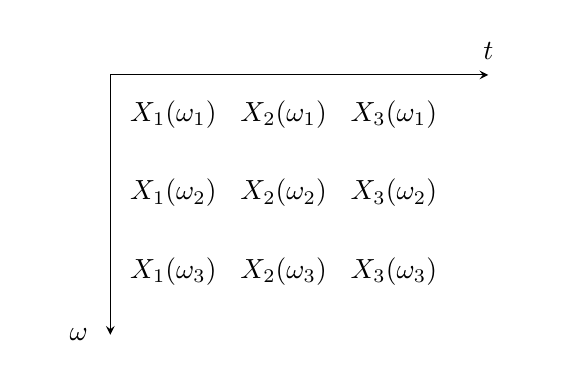
\begin{tikzpicture}[scale = 0.20]
    \definecolor{FFFFFF}{RGB}{255,255,255}
    \draw [draw=none] (37.0,-25.0) rectangle node(IDOL_J-3)[align = center, text width = 1.3 cm,inner sep=0] {$t$} (43.0,-28.0);
    \draw [draw=none] (11.0,-43.0) rectangle node(IDOL_J-4)[align = center, text width = 1.3 cm,inner sep=0] {$\omega$} (17.0,-46.0);
    \draw [draw=none] (17.0,-29.0) rectangle node(IDOL_J-5)[align = center, text width = 1.3 cm,inner sep=0] {$X_1(\omega_1)$} (23.0,-32.0);
    \draw [draw=none] (17.0,-34.0) rectangle node(IDOL_J-6)[align = center, text width = 1.3 cm,inner sep=0] {$X_1(\omega_2)$} (23.0,-37.0);
    \draw [draw=none] (17.0,-39.0) rectangle node(IDOL_J-7)[align = center, text width = 1.3 cm,inner sep=0] {$X_1(\omega_3)$} (23.0,-42.0);
    \draw [draw=none] (24.0,-29.0) rectangle node(ID_J-10)[align = center, text width = 1.3 cm,inner sep=0] {$X_2(\omega_1)$} (30.0,-32.0);
    \draw [draw=none] (24.0,-39.0) rectangle node(ID_J-12)[align = center, text width = 1.3 cm,inner sep=0] {$X_2(\omega_3)$} (30.0,-42.0);
    \draw [draw=none] (31.0,-29.0) rectangle node(ID_J-13)[align = center, text width = 1.3 cm,inner sep=0] {$X_3(\omega_1)$} (37.0,-32.0);
    \draw [draw=none] (31.0,-34.0) rectangle node(ID_J-14)[align = center, text width = 1.3 cm,inner sep=0] {$X_3(\omega_2)$} (37.0,-37.0);
    \draw [draw=none] (31.0,-39.0) rectangle node(ID_J-15)[align = center, text width = 1.3 cm,inner sep=0] {$X_3(\omega_3)$} (37.0,-42.0);
    \draw [draw=none] (24.0,-34.0) rectangle node(ID_J-23)[align = center, text width = 1.3 cm,inner sep=0] {$X_2(\omega_2)$} (30.0,-37.0);
    \draw [-stealth,solid](16.0,-28.0)--(40.0,-28.0);
    \draw [-stealth,solid] (16.0,-28.0) -- (16.0,-44.5);
\end{tikzpicture}
}
    \caption{A Sample Space for a Stochastic Process}
\end{figure}

\begin{remark}
    \textbf{In the following two process, it is essential to distinguish ``measure by time'' and ``measure by successes'', e.g., given a number of successes, how long does it take to achieve them, or given a time interval, how many successes are achieved.}
\end{remark}

\section{Bernoulli Process}

\subsection{Definition and Properties}
\begin{definition}[Bernoulli Process]
    Bernoulli process is a sequence $X_1, X_2, \ldots$ of i.i.d. Bernoulli RVs $X_i$ with
    \begin{equation}
    \begin{aligned}
        \mathbf{P}(\text{success}) &= \mathbf{P}(X_i = 1) = p \\ 
        \mathbf{P}(\text{failure}) &= \mathbf{P}(X_i = 0) = 1 - p 
    \end{aligned}
    \end{equation}
    for each $i$.
\end{definition}
\begin{example}[Examples of Bernoulli Process]
    \begin{itemize}
        \item Sequence of lottery wins/losses
        \item Sequence of transistor qualified/unqualified
        \item Arrivals (each second) to a bank
        \item Arrivals (at each time slot) to server
    \end{itemize}
\end{example}
\begin{property}[Property of Bernoulli Process]
    \begin{itemize}
        \item \textbf{Independence:} For any given time $n$, the sequence of $X_{n+1}, X_{n+2}, \ldots$ is also a Bernoulli process, and is independent from $X_1, \ldots , X_n$.
        \item \textbf{Memoryless:}  Let $n$ be a given time and let $\overline{T}$ be the time of the first success after time $n$. Then $\overline{T} - n$ has a geometric distribution with parameter $p$, and is independent of the RVs $X_1, \ldots X_n$.
    \end{itemize}
\end{property}
\begin{proof}
    Let $\overline{T}$ be the first time after $n$ that $X_i = 1$. Then, the probability that $\overline{T} - n$, conditioning $n$, is given by
    \begin{equation}
        \mathbf{P}(\overline{T} - n = t \mid n) = \mathbf{P}(X_{n+1} = 0, X_{n+2} = 0, \ldots, X_{n+t-1} = 0, X_{n+t} = 1) = p(1-p)^{t-1} = \mathbf{P}(t)
    \end{equation}
\end{proof}

\begin{example}[Example of Memoryless Property]
    Let $N$ be the first $i$ for which $X_{i-1} = X_i = 1$. What is the probability $\mathbf{P}\qty(X_{N+1} = X_{N+2} = 0)$ that there are no successes in the two trials that follow?
\end{example}
\begin{solution}
    Use total probability theorem and memoryless property
    \begin{equation}
    \begin{aligned}
        \mathbf{P}(X_{N+1} = X_{N+2} = 0) &= \sum_{n=1}^{\infty} \mathbf{P}(X_{N+1} = X_{N+2} = 0 \mid N = n) \cdot \mathbf{P}(N = n) \\ 
        &= (1 - p)^2 \sum_{n=1}^{\infty} \mathbf{P}(N = n) = (1 - p)^2
    \end{aligned}
    \end{equation}
\end{solution}

\subsection{Interarrival Times}
Denote the time of the $k$-th success as $Y_k$, and the $k$-th interarrival time as $T_k$, that is 
\begin{equation}
    T_1 = Y_1, \quad T_k = Y_k - Y_{k-1}, \quad Y_k = T_1 + T_2 + \ldots + T_k
\end{equation}
According to the memoryless property, the interarrival times $T_k$ are i.i.d. geometric RVs with parameter $p$, which yields an alternative description of the Bernoulli process.
\begin{definition}[Alternative Description of the Bernoulli Process]
    \begin{enumerate}
        \item Start with a sequence of i.i.d. geometric RVs $T_1, T_2, \ldots$ with parameter $p$, and let these stand for the interarrival times.
        \item Record a success $X_i = 1$ at times $i = Y_k = T_1 + T_2 + \ldots + T_k$, otherwise record a failure $X_i = 0$.
        \item The sequence $X_i$ is then a Bernoulli process with parameter $p$.
    \end{enumerate}
\end{definition}

Also, we can measure the expectation and variance of the time until the $k$-th success, which is given by
\begin{align}
    \E\qty[Y_k] &= \sum_{i=1}^{k} \E\qty[T_i] = \frac{k}{p} \\
    \var\qty(Y_k) &= \sum_{i=1}^{k} \var\qty(T_i) = \frac{k(1-p)}{p^2}
\end{align}
Detailedly, the distribution of $Y_k$ is given by
\begin{equation}
    p_{Y_k}(t) = \binom{t-1}{k-1} p^k (1-p)^{t-k}
\end{equation}
meaning that the time until the $k$-th success is distributed as a negative binomial distribution with parameters $k$ and $p$, which can be proved as follows:
\begin{proof}
    For $t \geq k$, we observe that the event $\{Y_k = t\}$ will occur if and only if both of the following two events $A$ and $B$ occur:
    \begin{itemize}
        \item Event $A$: there is a success at time $t$.
        \item Event $B$: there are exactly $k-1$ successes in the first $t-1$ trials.
    \end{itemize}
    The probability of event $A$ and event $B$ is given by
    \begin{equation}
        \mathbf{P}(A) = p, \quad \mathbf{P}(B) = \binom{t-1}{k-1} p^{k-1} (1-p)^{t-k}
    \end{equation}
    Since $A$ and $B$ are independent, we have
    \begin{equation}
        \mathbf{P}(Y_k = t) = \mathbf{P}(A) \cdot \mathbf{P}(B) = \binom{t-1}{k-1} p^k (1-p)^{t-k}
    \end{equation}
\end{proof}

\subsection{Splitting and Merging}
For a Bernoulli process with parameter $p$, whenever there is a success, we can split success into process $A$ or process $B$ (mutually exclusively) with probabilities $p_A$ and $p_B$, respectively, where $p_A + p_B = 1$; whenever there is a failure, we record it as a failure in both processes. The resulting processes $A$ and $B$ are also Bernoulli processes with parameters $p\cdot p_A$ and $p \cdot p_B$, respectively. The proof is obvious. \textbf{Non of the three processes are independent point-wise, but the two resulting processes $A$ and $B$ are independent as a whole. (Futher studying in course ``Probability and Stochastic Processes (2)'')}
\begin{figure}[H]
    \centering
    \includegraphics[width=0.4\linewidth]{images/Note-13.3.png}
    \caption{Splitting a Bernoulli Process}
\end{figure}

For two independent Bernoulli processes $A$ and $B$ with parameters $p_A$ and $p_B$, respectively, whenever there is a success in either process, we record it as a success in the merged process $C$, otherwise we record it as a failure. The resulting process $C$ is also a Bernoulli process with parameter $p_A + p_B - p_A \cdot p_B$.  The proof is also obvious. \textbf{The resulting process $C$ is not independent point-wise from the two original processes $A$ and $B$, but it is independent as a whole. (Futher studying in course ``Probability and Stochastic Processes (2)'')}
\begin{figure}[H]
    \centering
    \includegraphics[width=0.4\linewidth]{images/Note-13.2.png}
    \caption{Merging Two Bernoulli Processes}
\end{figure}


\section{Poisson Process}
\subsection{Definition and Properties}
\begin{definition}[Poisson Process]
    An arrival process is called a Poisson process with parameter $\lambda$ if it satisfies the following properties:
    \begin{itemize}
        \item \textbf{Time homogeneity:} The probability of the number of arrivals $k$ only depends on the length of the time interval, not the absolute time.
        \begin{equation}
            \mathbf{P}(k, t) = \mathbf{P}(k \text{ events in \textbf{interval of duration} } t)
        \end{equation}
        \item \textbf{Independence:} The number of arrivals in disjoint time intervals are independent.
        \item \textbf{Small interval probabilities:} 
        \begin{equation}
            \mathbf{P}(k, t) = \left\{\begin{aligned}
                & 1 - \lambda t + o(t) &\quad k = 0 \\
                & \lambda t + o_1(t) &\quad k = 1 \\
                & o_2(t) &\quad k \geq 2
            \end{aligned}\right.
        \end{equation}
    \end{itemize}
\end{definition}

By dividing the total time interval $t$ into $n$ small intervals of length $\delta = t/n$, we can use Bernoulli process to approximate the Poisson process. Finally, we can take the limit as $n \to \infty$ to obtain $\mathbf{P}(k, t)$.
\begin{figure}[H]
    \centering
    \includegraphics[width=0.6\linewidth]{images/Note-13.4.png}
    \caption{Poisson Process as a Limit of Bernoulli Process}
\end{figure}

In each small interval, the probability of having one arrival is $\lambda \delta$ (ignoring the $o(\delta)$ term, as when we take the sum of all small intervals, $o(\delta)$ will become $o(t)$, which is also a small term). Ignore the probability of having more than one arrival in each small interval.
As all the small intervals are independent, the total number of arrivals in the total time interval $t$ approximately follows a binomial distribution with parameters $n$ and $p = \lambda \delta = \lambda t/n$. 
\begin{equation}
\begin{aligned}
    \mathbf{P}(k, t) &= \lim_{n \to \infty} \binom{n}{k} p^k (1-p)^{n-k} = \lim_{n \to \infty} \frac{n!}{(n-k)! k!} \cdot p^k (1-p)^{n-k} \\
    &= \lim_{n \to \infty} \frac{n(n-1)(n-2)\cdots(n-k+1)}{k!} \cdot \qty(\frac{\lambda t}{n})^k \cdot \qty(1 - \frac{\lambda t}{n})^{n-k} \\
    &= \lim_{n \to \infty} \frac{n(n-1)(n-2)\cdots(n-k+1)}{n^k} \cdot \frac{(\lambda t)^k}{k!} \cdot \qty(1 - \frac{\lambda t}{n})^{n-k} \\\
    &= 1 \cdot \frac{(\lambda t)^k}{k!} \cdot \e^{-\lambda t} = \frac{(\lambda t)^k}{k!} \e^{-\lambda t}
\end{aligned}
\end{equation}

Let $N_t$ be the number of arrivals in the time interval $t$, then $p_{N_t}(k) = \mathbf{P}(N_t = k) = \mathbf{P}(k, t)$, which is a Poisson distribution with parameter $\lambda t$, that is
\begin{equation}
    N_t \sim \text{Poisson}(\lambda t), \quad \E[N_t] = \lambda t, \quad \var(N_t) = \lambda t
\end{equation}
\begin{example}[Example of Poisson Process]
    In an area, the occurrences of target objects follow a Poisson process with a rate of $\lambda = 0.2$ occurrences per hour. The radar continuously detects objects, and the monitor checks the number of detections every hour. What is the probability of getting 0 and 1 new detections during each check?
\end{example}
\begin{solution}
    $N_t \sim \text{Poisson}(0.2t)$. For $t = 1$ hour, we have
    \begin{equation}
        \mathbf{P}(N_1 = 0) = \e^{-0.2} \approx 0.819, \quad \mathbf{P}(N_1 = 1) = 0.2 \e^{-0.2} \approx 0.164
    \end{equation}
\end{solution}

\subsection{Interarrival Times}
We first find out the distribution of the first arrival time $T_1$, and then we can use the memoryless property to find the distribution of the interarrival times $T_k$, and finally $Y_k$.

For the first arrival time $T_1$, we have
\begin{align}
    F_{T_1}(t) &= \mathbf{P}(T_1 \leq t) = 1 - \mathbf{P}(T_1 > t) = 1 - \mathbf{P}(N_t = 0) = 1 - \e^{-\lambda t}, \quad t \geq 0 \\ 
    f_{T_1}(t) &= \dv{t} F_{T_1}(t) = \lambda \e^{-\lambda t}, \quad t \geq 0 \\ 
    \E[T_1] &= \frac{1}{\lambda}, \quad \var(T_1) = \frac{1}{\lambda^2}
\end{align}
Thus $T_1$ follows an exponential distribution with parameter $\lambda$, which has the \textbf{Memoryless Property: The time to the next arrival is independent of the past.}

Denote the time of the $k$-th arrival as $Y_k = T_1 + T_2 + \ldots + T_k$, where $T_i$ are i.i.d. exponential RVs with parameter $\lambda$, which yields an alternative description of the Poisson process, just like the Bernoulli process.
\begin{definition}[Alternative Description of the Poisson Process]
    \begin{enumerate}
        \item Start with a sequence of i.i.d. exponential RVs $T_1, T_2, \ldots$ with parameter $\lambda$, and let these stand for the interarrival times.
        \item Record an arrival at times $i = Y_k = T_1 + T_2 + \ldots + T_k$, otherwise record a failure.
        \item The sequence $N_t$ is then a Poisson process with parameter $\lambda$.
    \end{enumerate}
\end{definition}
Also, we can measure the expectation and variance of the time until the $k$-th arrival, which is given by
\begin{align}
    \E\qty[Y_k] &= \sum_{i=1}^{k} \E\qty[T_i] = \frac{k}{\lambda} \\
    \var\qty(Y_k) &= \sum_{i=1}^{k} \var\qty(T_i) = \frac{k}{\lambda^2}
\end{align}
Detailedly, the distribution of $Y_k$ is given by
\begin{equation}
    f_{Y_k}(t) = \frac{\lambda^k t^{k-1} \e^{-\lambda t}}{(k-1)!}, \quad t \geq 0
\end{equation}
which is called the Erlang distribution with parameters $k$ and $\lambda$, which can be proved as follows:
\begin{proof}
    For $t \geq 0$, we observe that the $k$-th arrival in time interval $[t, t + \delta]$ if and only if both of the following two events $A$ and $B$ occur:
    \begin{itemize}
        \item Event $A$: there are exactly $k-1$ arrivals in the interval $[0, t]$.
        \item Event $B$: there is one arrival in the interval $[t, t + \delta]$.
    \end{itemize}
    The probability of event $A$ and event $B$ is given by
    \begin{equation}
        \mathbf{P}(A) = \frac{(\lambda t)^{k-1} \e^{-\lambda t}}{(k-1)!}, \quad \mathbf{P}(B) = \lambda \delta + o_1(\delta)
    \end{equation}
    Since $A$ and $B$ are independent, we have
    \begin{equation}
        \delta f_{Y_k}(t) = \mathbf{P}(t \leq Y_k \leq t + \delta) = \mathbf{P}(A) \cdot \mathbf{P}(B) = \frac{(\lambda t)^{k-1} \e^{-\lambda t}}{(k-1)!} \cdot (\lambda \delta + o_1(\delta))
    \end{equation}
    Ignore the $o_1(\delta)$ term, we have
    \begin{equation}
        f_{Y_k}(t) = \frac{\lambda^k t^{k-1} \e^{-\lambda t}}{(k-1)!}, \quad t \geq 0
    \end{equation}
\end{proof}
\begin{example}[Example of Erlang Distribution]
    In a single-cycle processor, there are 56 instructions waiting to be processed. The processor processes instructions at a rate of $\lambda = 2$ per $\mu$s. How long will it take for all instructions to be processed, and what is the probability that the processing time will exceed 30 $\mu$s?
\end{example}
\begin{solution}
    The processing time in $\mu$s, defined as $Y$, is Erlang of order 56.
    \begin{equation}
        \E[Y] = \frac{56}{\lambda} = \frac{56}{2} = 28
    \end{equation}
    The probability that the processing time exceeds 30 $\mu$s is given by
    \begin{equation}
        \mathbf{P}(Y > 30) = 1 - F_Y(30) = \int_{30}^{\infty} \frac{\lambda^{56} t^{55} \e^{-\lambda t}}{55!} \dd{t}
    \end{equation}
\end{solution}

\subsection{Splitting and Merging}
For a Poisson process with parameter $\lambda$, whenever there is an arrival, we can split it into process $A$ or process $B$ (mutually exclusively) with probabilities $p_A$ and $p_B$, respectively, where $p_A + p_B = 1$; whenever there is no arrival, we record it as a failure in both processes. The resulting processes $A$ and $B$ are also Poisson processes with parameters $\lambda \cdot p_A$ and $\lambda \cdot p_B$, respectively. \textbf{Non of the three processes are independent point-wise, but the two resulting processes $A$ and $B$ are independent as a whole. (Futher studying in course ``Probability and Stochastic Processes (2)'')}
\begin{proof}
    For process $A$ (process $B$ can be proved similarly)
    \begin{equation}
    \begin{aligned}
        \mathbf{P}(N_At = k) &= \sum_{n=k}^{\infty} \mathbf{P}(N_t = n) \cdot \binom{n}{k} p_A^k (1-p_A)^{n-k} = \cdots \\ 
        &= \frac{\exp\qty(-\lambda t p_A)(\lambda t p_A)^k}{k!} \sum_{n=k}^{\infty} \frac{\exp\qty(\lambda t(p_A-1)) (\lambda t(1-p_A))^{n-k}}{(n-k)!} \\ 
        &= \exp\qty(-\lambda t p_A) \cdot \frac{(\lambda t p_A)^k}{k!}
    \end{aligned}
    \end{equation}
\end{proof}

For two independent Poisson processes $A$ and $B$ with parameters $\lambda_A$ and $\lambda_B$, respectively, whenever there is an arrival in either process, we record it as an arrival in the merged process $C$, otherwise we record it as a failure. The resulting process $C$ is also a Poisson process with parameter $\lambda_A + \lambda_B$. The proof is also obvious by definition. \textbf{The resulting process $C$ is not independent point-wise from the two original processes $A$ and $B$, but it is independent as a whole. (Futher studying in course ``Probability and Stochastic Processes (2)'')}
\begin{figure}[H]
    \centering
    \includegraphics[width=0.4\linewidth]{images/Note-13.5.png}
    \caption{Merging Two Poisson Processes}
\end{figure}

\appendix
\chapter{Problem Solutions}


\section{Derived Distributions}
\textbf{In the lecture right after I finished this section, the lecturer provided an ``official'' solution to this problem, see section \ref{sec:derived-distributions}.}

In the homework, I constantly encounter some problems like this:
\begin{example}[PDF of a Function of Multiple Continuous RVs]
    Let $X, Y$ be two continuous RVs with joint PDF $f_{X, Y}(x, y)$, and $Z = g(X, Y)$. Find the PDF of $Z$.
\end{example}

Here I introduce two approaches to solve this kind of problems: CDF and Jacobian transformation.
\begin{solution}
    \textbf{CDF:}
    \begin{enumerate}
        \item Find the CDF of $Z$
            \begin{equation}
                F_{Z}(z) = \mathbf{P}(Z \leq z) = \mathbf{P}(g(X, Y) \leq z) = \iint_{g(x, y) \leq z} f_{X, Y}(x, y) \dd{x} \dd{y}
            \end{equation}
        \item Differentiate $F_{Z}(z)$ to get the PDF of $Z$
            \begin{equation}
                f_{Z}(z) = \dv{F_{Z}(z)}{z}
            \end{equation}
    \end{enumerate}
\end{solution}
\begin{solution}
    \textbf{Jacobian Transformation:} This approach requires finding a valid variable substitution with invertibility. \\ 
    Take $Z = g(X, Y) = X + Y$ as an example. Normally, if we want to calculate the determinant of the Jacobian matrix, the Jacobian matrix must be square. However, here $Z$ is a scalar instead of a vector. We take the following steps to avoid this problem:
    \begin{enumerate}
        \item Let $U = X + Y$ and $V = X$, then $X = V$ and $Y = U - V$.
        \item Calculate the Jacobian matrix and its determinant
            \begin{align}
                &J = \mqty(\pdv{X}{U} & \pdv{X}{V} \\ \pdv{Y}{U} & \pdv{Y}{V}) = \mqty(0 & 1 \\ 1 & -1) \\ 
                &\det(J) = -1 
            \end{align}
        \item Find the joint PDF of $U$ and $V$
            \begin{equation}
                f_{U, V}(u, v) = f_{X, Y}(v, u - v) \cdot \abs{\det(J)} = f_{X, Y}(v, u - v)
            \end{equation}
        \item Integrate out $V$ to get the marginal PDF of $U$, which is the PDF of $Z$
            \begin{equation}
                f_{U}(u) = \int_{-\infty}^{+\infty} f_{X, Y}(v, u - v) \dd{v}
            \end{equation}
    \end{enumerate}
\end{solution}



\end{document}
